%% The openany option is here just to remove the blank pages before a new chapter
\documentclass[11pt,openany]{book}
\usepackage[utf8]{inputenc}
\usepackage[utf8]{vietnam}
\usepackage{subcaption}
\usepackage{graphicx}
\usepackage{kantlipsum}
\usepackage{amsfonts}
\usepackage{amsmath}
\usepackage{float}
\usepackage{algorithm}
\usepackage{algorithmic}
\usepackage{hyperref}
\usepackage{tabularx}
\usepackage{diagbox}
\usepackage{slashbox}
\usepackage{lscape}
\usepackage{multirow}
\usepackage{longtable}
\usepackage{biblatex}
\addbibresource{mybib.bib}
\title{Communicating Multi-UAV System for cooperative SLAM-based Exploration}

\usepackage{pagenote}
\setcounter{chapter}{0}

%% End notes to be printed as sections at the
%% end of each chapter.
\renewcommand*{\notedivision}{\section*{\notesname}}
\renewcommand*{\pagenotesubhead}[1]{}


%%%%%%%%%%%%% For customising the endnote markers. Comment these out if you don't want them.
% To prefix each note number with the chapter number
\renewcommand{\thepagenote}{\thechapter-\arabic{pagenote}}

% To have a slightly different formatting for the endnote numbers in the text -- smaller text, sans-serif, square brackets
\renewcommand\notenumintext[1]{\space{\footnotesize\sffamily[FN-#1]}}

% To have a slightly different formatting for the endnote numbers in the notes section. Just the square brackets and sans-serif; normal size.
\renewcommand\notenuminnotes[1]{{\sffamily[FN-#1] }}

% If you want a different name/heading for the end notes
\renewcommand{\notesname}{End Notes}
%%%%%%%%%%%%% End customisation

%% THIS LINE IS MANDATORY
\makepagenote

\begin{document}
\begin{titlepage}
    \begin{center}
        \small
        TRƯỜNG ĐẠI HỌC BÁCH KHOA HÀ NỘI\\
        \vspace{0.2cm}
        \LARGE
        \textbf{VIỆN ĐIỆN TỬ - VIỄN THÔNG}\\
        \vspace{1.5cm}
        
\includegraphics[scale=0.3]{assets/logo.png}\\
        \vspace{1.5cm}
        \LARGE
        BÁO CÁO GIỮA KỲ\\
        \vspace{0.5cm}
        \Huge
        \textbf{ĐIỆN TỬ TƯƠNG TỰ II \\ DỊCH TÀI LIỆU}
        \vspace{1cm}
        \Large
        \begin{center}
            \begin{tabular}{ l l }
                \textbf{Nhóm}        & 49            \\
                \textbf{Sinh viên 1} & Tạ Hoàng Việt \\
                                     & 20172916      \\
                \textbf{Sinh viên 2} & Hồ Huy Hoàng  \\
                                     & 20172581
            \end{tabular}
        \end{center}
        \vspace{1cm}
        \normalsize
        Hà Nội, 06/2021
    \end{center}
\end{titlepage}
\tableofcontents
\listoffigures
\listoftables
\newpage
\thispagestyle{plain}
\addcontentsline{toc}{chapter}{Introduction}
\begin{center}
    \Huge
    \textbf{Introduction}
\end{center}
% TODO: add introduction here
\chapter{Coordinated exploration}
\section{Introduction}
The exploration and mapping of large areas is an active field of research in aerial robotics. It consists in constructing a 3D model representation of the workspace as robots progress within it. Recently, the key subject in the exploration problem is the cooperative deployment of fleet of robots that promise enhanced performances compared to single robot exploration.\\\\
In this chapter, we address the problem of cooperative exploration strategies with no a- priori knowledge of the environment. We will try to answer the question: Where should each robot move next?
\section{Related work}
Recently, several works have proposed solutions for exploration using multi-robot teams to reduce the mission time and to increase the scalability \cite{bautin2012strategie}, \cite{jensen2013rolling}, \cite{yan2014team}. Hence, the challenge is to have an efficient cooperation among the agents in the fleet while maintaining communication \cite{rooker2007multi}. For that, existing approaches can be centralized, that is, one robot in the fleet is responsible for assigning targets \cite{burgard2000collaborative}. In \cite{schmuck2017multi}, a central server with increased computational resources is adopted to receive, treat, optimize and send back information to other robots. Other works, such as \cite{yuan2010cooperative},\cite{sheng2006distributed}, use distributed approaches where each robot chooses its own target. Another trend is to switch from individual to cooperative exploration behavior when robots are not able to converge to a local minimum at a satisfying rate \cite{wu2012robust}. In \cite{konolige2003map}, authors propose to consider four possibilities taking into account robots’ interactions in order to construct a distributed map. The situations involved are: no interaction (robots are not within each others’ communication range), hypothesis generation (there is an interaction between the robots but they do not know their respective location), hypothesis verification (there is an interaction between the robots and they propose an hypothesis about their location), and coordinated exploration (there is an interaction between robots and they do share their maps).
\subsection{Robot-to-target assignment}
The mapping algorithm is performed while a robot attempts to reach a target. So, for an effective environment mapping, the target should be chosen carefully. There is a wide variety of goal assignment strategies to affect one robot to a target. The majority of them are centralized and use a cost function to compute the utility of reaching a target.\\\\
In the greedy assignment \cite{yamauchi1998frontier}, each robot chooses a target depending on its cost function without coordinating with other robots. Hence, one target can be visited by different robots. To solve this issue, already chosen targets can be discarded before being considered for assignment by others using Broadcast of Local Eligibility (BLE) \cite{werger2000broadcast} also called Iterative Assignment. But, this method does not necessarily produce the optimal solution since it depends on the order of robots.\\\\
The K-means method \cite{solanas2004coordinated} consists in dividing the environment to explore into regions of the same number of robots, then, assigning one robot to the closest region where it will choose a target from the frontiers depending on a cost function.\\\\
The Hungarian method \cite{deb1999multi} proposed by \cite{kuhn2005hungarian}, solves the worker- task assignment written in the form of $n \times n$ matrix $C$ where $c_{i,j}$ is the cost of the task $j$ assigned to the worker $i$. The optimal assignment is found with time complexity $O(n^3)$. This algorithm requires that the number of workers is equal to the number of tasks which cannot be guaranteed. Else, imaginary robots or targets can be added to satisfy the assumption, and skipped later in the selection.\\\\
Authors in \cite{nanjanath2006dynamic} present an auction-based method to assign tasks to a group of robots. The distribution of tasks is accomplished by means of a first-price reverse auction which means that the auctioneer is the buyer. One task is auctioned one at a time by priority. Then, the auctioneer selects the best bid and assigns the task to the corresponding bidder. The algorithm is well adapted to dynamic environments, where unexpected obstacles might prevent a robot from reaching its target.\\\\
In \cite{zhao1996genetic}, \cite{leigh2007using}, a genetic algorithm is used to optimally assign robot to tasks. It is an NP-hard problem since it is considered as a generalized two- dimensional multi-type bin packing problem.\\\\
Authors in \cite{faigl2012goal} present a new approach called Multiple Traveling Salesman Problem (MTSP) for robot-to-target assignment in multi-robot exploration problem. It consists in clustering an environment, determining the cost of TSP distance for each pair of robot cluster, assigning goals from non empty cluster, and finally fixing goals for empty clusters. This approach was compared with greedy, iterative and Hungarian method. The MTSP presents competitive results regarding the total computational requirements and the increasing number of robots.\\\\
In \cite{kulich2015comparison}, a comparison of some assignment strategy used for multi- robot system is done. The compared strategies include Hungarian method, Greedy, BLE method and K-means clustering. Results show that Hungarian method outperforms other approaches in majority of cases. Unlike the Hungarian method, the iterative assignment can be implemented in a distributed environment. Also the Hungarian methods are computationally heavy compared with the simple greedy algorithm which is preferred in applicable scenario.
\subsection{Utility function}
Most of the robot-to-target assignments are based on an utility function that defines the benefits that a robot have to reach this target, taking into account the mission’s aim \cite{burgard2000collaborative}. The work proposed in \cite{benavides2016multi} presents a new utility function that takes into account the traveling cost to the target and the connectivity utility. This allows a trade off between minimizing the amount of exploration time and the connectivity. To speed up velocity, authors in \cite{cieslewski2017rapid} propose a rapid frontier selection technique to select goals from the robot’s field of view. This approach minimizes the overall mission time by minimizing the change in velocity of the robot. Nonetheless, this approach increases the total path length traveled. In \cite{heng2015efficient}, maximizing the reconstructed model is favored over the mission time. Furthermore, the proposed approach solves simultaneously exploration and coverage problems in order to maximize the completeness of the reconstructed model. Whereas in \cite{simmons2000coordination}, the aim is the maximization of the utility of targets that minimizes the potential for overlap in information gain amongst members of the fleet. The utility of reaching a target depends basically on the aim of the mission while taking into account some additional constraints such as time, completeness of the map, limited sensor and communication range, or number of robots.
\section{Proposed exploration strategy}
\subsection{Overview}
In a Multi-UAV system, the exploration strategy needs to be cooperative to maximize the efficiency. The main objective proposed here, is to cooperatively choose specific regions to be simultaneously explored using a frontier-based approach. Commonly, this is done by selecting candidate targets and assigning them to each robot in an optimized manner. Figure \ref{fig:3.1} shows the proposed pipeline exploration process performed by each UAV.
\begin{figure}[H]
    \centering
    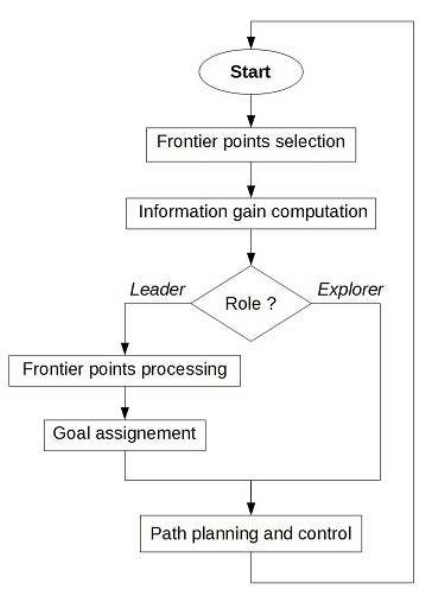
\includegraphics[scale=0.6]{assets/3_1.png}
    \caption{Proposed exploration process pipeline.}
    \label{fig:3.1}
\end{figure}
Each UAV selects the frontier points of its constructed local map during the SLAM step. Then, it computes the corresponding information gain of these points. If the UAV’s role is an \textit{explorer}, it would passively wait until receiving instructions; else, if it acts as a \textit{leader}, it would process the collected frontier points, and would assign a target to each robot in the group. Given a target, UAVs will plan a specific path to reach it.\\\\
During these steps, the map structure evolves from a projected 2D grid map obtained from the localization and mapping module, through frontier points during the frontier selection process, then candidate targets during the frontier processing step, to a final set of selected targets to reach. The evolution of the map structure is illustrated in Figure \ref{fig:3.2}. Algorithm \ref{alg:3.1} describes the main steps performed during the exploration.
\begin{algorithm}
    \caption{Exploration strategy for coordinated Multi-UAV}
    \label{alg:3.1}
    \begin{algorithmic}[1]
        \STATE From cell $\mathbf{l}_l \in \mathcal{L}$, select frontier points $\mathbf{f}_{i,j} \in \mathcal{F}$ and compute their respective information gain $\mathit{\mathbf{I}}(\mathbf{f}_{i,j})$.
        \STATE Process frontier points $\mathbf{f}_{i,j}$ to get candidate goals $\mathbf{t}_k \in \mathcal{G}$ (See Algorithm \ref{alg:3.2})
        \STATE Assign UAV$_i$ with target $k$ (See Algorithm \ref{alg:3.2}).
        \STATE Send targets to the corresponding robots.
    \end{algorithmic}
\end{algorithm}
\begin{figure}[H]
    \centering
    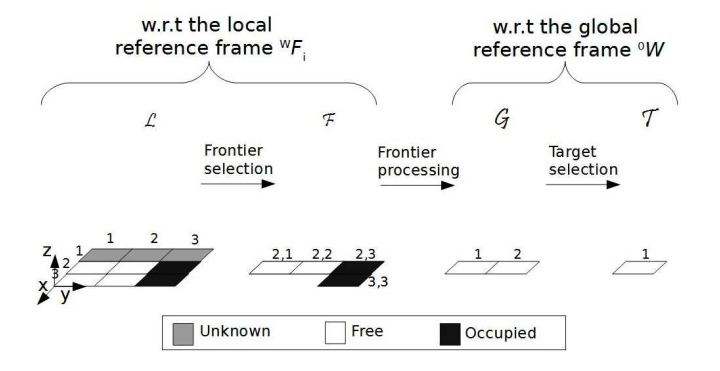
\includegraphics[scale=0.4]{assets/3_2.png}
    \caption{Map structure evolution during the exploration process: From 2D cells $\mathcal{L}$ to 2D frontier cells $\mathcal{F}$ to candidate frontier cells/points $\mathcal{G}$ (candidate targets) to 2D target cells/points $\mathcal{T}$.}
    \label{fig:3.2}
\end{figure}
\subsection{Frontier points selection}
The frontier selection process is used to define the frontiers of regions bounded by obstacles or unknown spaces (See Figure \ref{fig:3.3}).
\begin{figure}[H]
    \centering
    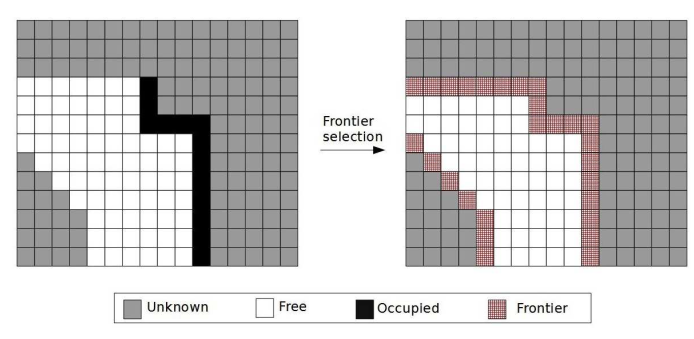
\includegraphics[scale=0.4]{assets/3_3.png}
    \caption{Frontier cells/points selection of a 2D occupancy grid map.}
    \label{fig:3.3}
\end{figure}
The frontier cells $\mathbf{f}_{i,j} \in \mathcal{F}$ are selected from the set of cells $\mathcal{L}(\mathcal{F}\subset \mathcal{L})$ such that they are either:
\begin{itemize}
    \item Free $\mathbf{l}_f$ and adjacent to unknown.
    \item Labeled as occupied $\mathbf{l}_o$ . The Occupied cells $\mathbf{l}_o$ are considered as frontier cells to be able to perform frontier processing in the next step. They could not be chosen as target and will be discarded later.
\end{itemize}
In Figure \ref{fig:3.2}, the frontier cells are: $\mathbf{l}_f(2,1)$,$\mathbf{l}_f(2,2)$ , $\mathbf{l}_f(2,3)$, and $\mathbf{l}_f(3,3)$. Thus, for a cluster $\mathcal{C}$ containing UAV$_i$ , the frontiers are:
\begin{equation} \label{eq:3.1}
    \mathcal{F}=\{\mathbf{f}_{i,1}(2,1),\mathbf{f}_{i,2}(2,2),\mathbf{f}_{i,3}(2,3),\mathbf{f}_{i,4}(3,3)\}
\end{equation}
\subsection{Information gain computation}
In frontier-based exploration approaches, only cells adjacent to unknown ones may be defined as candidate frontier points and are likely to be chosen as targets. Thereby, the information gain is associated to each of them in order to estimate the utility of reaching each frontier. This corresponding information gain can be defined in different manners depending on the mission purpose. Authors in \cite{burgard2005coordinated} propose to use a probability function to reduce an assigned constant value taking into account the relative distance to the UAV’s pose. This strategy is general and does not take into account the updated explored cells. The approach proposed in \cite{heng2015efficient} affects, to the information gain, the number of unknown and not occluded cells in the view frustum of the target. This method depends on the real estimate of information gained when visiting the considered pose. However, it requires more computation.\\\\
In the proposed strategy, the information gain is allocated so that it defines the amount of unknown cells surrounding the target (See Figure \ref{fig:3.4}). It is a non-metric value that counts the number of cells labeled as unknown l u from the 48 cells around the frontier point.
\begin{figure}[H]
    \centering
    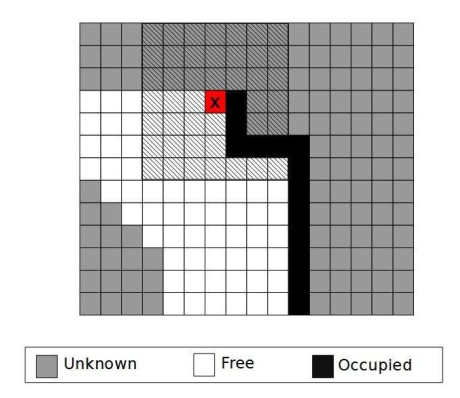
\includegraphics[scale=0.4]{assets/3_4.png}
    \caption{The information gain computation of a frontier point x (in red). The hatched cells represent the 48 surrounding cells of the frontier point \textbf{x}. The information gain of \textbf{x} is: $\mathbf{I}(x)=25$.}
    \label{fig:3.4}
\end{figure}
\subsection{Frontier points processing}
All frontier points $\mathbf{f}_{i,j} \in \mathcal{F}$ of UAV$_i$ in the cluster $\mathcal{C}$ with $i \in [1..n_c]$, are collected. Points in $\mathcal{F}$ are then processed using Algorithm \ref{alg:3.2} to get candidate frontier points considered as candidate targets $\mathbf{t}_k \in \mathcal{G}$ with $k \in [1..n_g]$ (See Figure \ref{fig:3.2})
\begin{algorithm}[H]
    \caption{Frontier processing algorithm.}
    \label{alg:3.2}
    \hspace*{\algorithmicindent} \textbf{Input:} Frontier points $\mathbf{f}_{i,j} \in \mathcal{F}$ of UAV$_i$ with $i \in [1..n_c]$. \\
    \hspace*{\algorithmicindent} \textbf{Output:} Candidate targets $\mathcal{G}$
    \begin{algorithmic}[1]
        \STATE $p_u=\cup_{i=1}^{n_c}\mathbf{f}_{i,j}$.
        \STATE $p_i=\cap_{i=1}^{n_c}\mathbf{f}_{i,j}$.
        \STATE $\mathcal{G}=p_u\setminus p_i$.
        \STATE Delete the obstacle frontier points $\mathbf{f}_{i,j}(x,y)=\mathbf{l}_o(x,y)$ from $\mathcal{G}$.
        \RETURN $\mathcal{G}$.
    \end{algorithmic}
\end{algorithm}
Figure \ref{fig:3.5} shows an example of frontier processing with two UAVs’ map to get the candidate targets. The obstacle frontier points $\mathbf{f}_{i,j}(x,y)=\mathbf{l}_o(x,y)$ – labeled as occupied – are only kept to compute the intersection of frontier points. Only the free frontier cells $\mathbf{l}_f$ can be considered as candidate target.\\\\
When using local frontier points instead of local maps, the frontier process replaces the map matching process where the aim is to clear overlapping areas. Hence, in the frontier processing step, the frontier points that belong to overlapping areas are cleared. Therefore, using frontier points allows important memory saving. To compute the frontier points that belong to the overlapped areas (Steps 1, 2 and 3 in Algorithm \ref{alg:3.2}), we propose two approaches with convex shapes and concave shapes assumptions.
\subsubsection{First approach: Convex shape map}
In this approach, map shapes are considered convex, which simplifies the intersection computation in Algorithm \ref{alg:3.3}. Figure \ref{fig:3.6} shows two examples of applying frontier processing algorithm while assuming convex shapes with two and three UAVs’ map.\\\\
This algorithm is relatively easy to apply, but results show that it does not perform well. The convex assumption leads to some false overlapped frontier points. Consequently, some unknown areas will not be visited since their corresponding points are removed and, thus, will not be assigned as a target.
\subsubsection{Second approach: Concave shape map}
In the second approach, we make the assumption of concave shapes for the UAVs’ map to compute their intersection in Algorithm \ref{alg:3.4}. Figure \ref{fig:3.7} shows two examples of applying frontier processing algorithm while assuming convex shapes with two and three UAVs’ map.
\begin{figure}[H]
    \centering
    \begin{subfigure}[H]{0.6\linewidth}
        \centering
        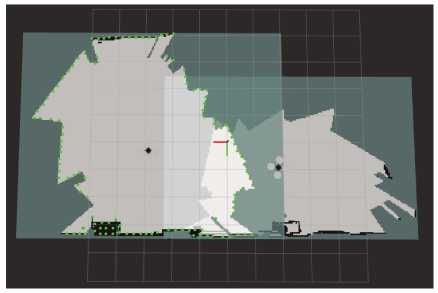
\includegraphics[width=\linewidth]{assets/3_5_a.png}
        \caption{{Frontiers $\mathbf{f}_{1,j}$ of UAV$_1$}}
        \label{fig:3.5a}
    \end{subfigure}
    \begin{subfigure}[H]{0.6\linewidth}
        \centering
        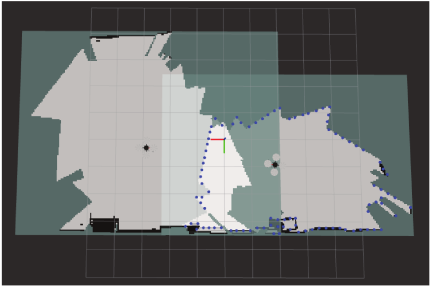
\includegraphics[width=\linewidth]{assets/3_5_b.png}
        \caption{{Frontiers $\mathbf{f}_{2,j}$ of UAV$_2$}}
        \label{fig:3.5b}
    \end{subfigure}
    \begin{subfigure}[H]{0.6\linewidth}
        \centering
        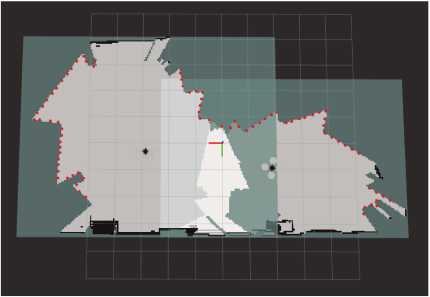
\includegraphics[width=\linewidth]{assets/3_5_c.png}
        \caption{{Candidate targets $\mathcal{G}$}}
        \label{fig:3.5c}
    \end{subfigure}
    \caption{Frontier points processing example: (a) and (b) represent the frontier points of UAV$_1$ and UAV$_2$, respectively. (c) represent the candidate targets. The process consists in removing frontier points that belong to overlapped areas, and those that are adjacent to obstacles.}
    \label{fig:3.5}
\end{figure}
\begin{algorithm}[H]
    \caption{Intersection computation algorithm with convex shapes assumption.}
    \label{alg:3.3}
    \hspace*{\algorithmicindent} \textbf{Input:} $Vect1, Vect2$ \\
    \hspace*{\algorithmicindent} \textbf{Output:} $Vect\_Final$
    \begin{algorithmic}[1]
        \FOR {$i \in Vect1$}
        \STATE $inf = 0, sup = 0$
        \FOR{ $j \in Vect2$}
        \IF {$Vect1(i).x < Vect2(i).x$}
        \STATE $inf++$;
        \ELSE
        \STATE $sup++$;
        \ENDIF
        \ENDFOR
        \IF {$inf>0$ and $sup>0$}
        \STATE $Vect\_inter.push\_back(Vect1(i))$
        \ENDIF
        \ENDFOR
        \FOR{$i \in Vect\_inter$}
        \STATE $inf=0,sup=0$;
        \FOR{$j \in Vect2$}
        \IF {$|Vect\_inter(i).x-Vect2(i).x| <0.5$}
        \STATE $inf++$;
        \ELSE
        \STATE $sup++$;
        \ENDIF
        \ENDFOR
        \IF {$inf>0$ and $sup>0$}
        \STATE $Vect\_Final.push\_back(Vect\_inter(i))$
        \ENDIF
        \ENDFOR
    \end{algorithmic}
\end{algorithm}
\begin{figure}[H]
    \centering
    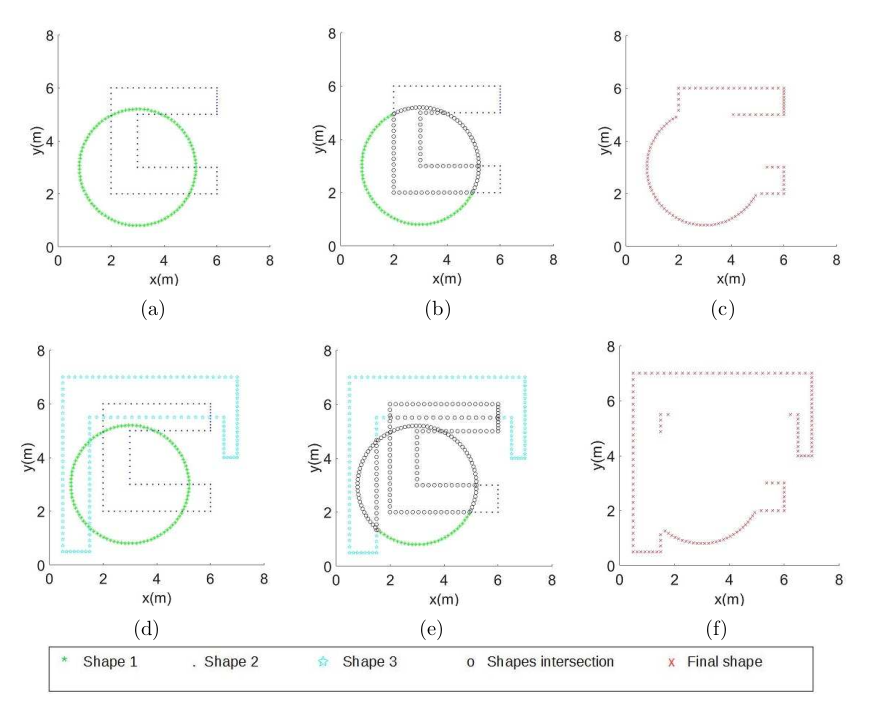
\includegraphics[scale=0.4]{assets/3_6.png}
    \caption{Frontier points processing wile assuming two convex map shapes in the first line and three in the second line. (a) and (d) represent two and three convex map shapes, respectively; (b) and (e) represent the frontier points in overlap (intersection); and (c) and (f) represent the obtained frontier points after processing (final shape).}
    \label{fig:3.6}
\end{figure}
\begin{algorithm}[H]
    \caption{Intersection computation algorithm with convex shapes assumption.}
    \label{alg:3.4}
    \hspace*{\algorithmicindent} \textbf{Input:} $Vect1, Vect2$ \\
    \hspace*{\algorithmicindent} \textbf{Output:} $Vect\_Final$
    \begin{algorithmic}[1]
        \FOR {$i \in Vect1$}
        \STATE $inf = 0, sup = 0$
        \FOR{ $j \in Vect2$}
        \IF {$Vect1(i).x < Vect2(i).x -0.5$}
        \STATE $inf++$;
        \ELSIF {$Vect1(i).x>Vect2(i).x+0.5$}
        \STATE $sup++$;
        \ELSE
        \STATE $eq++$;
        \ENDIF
        \ENDFOR
        \IF {$inf>0$ and $sup>0$ or $eq>0$}
        \STATE $Vect\_inter.push\_back(Vect1(i))$
        \ENDIF
        \ENDFOR
        \FOR{$i \in Vect\_inter$}
        \STATE $inf=0,sup=0, eq=0$;
        \FOR{$j \in Vect2$}
        \IF {$|Vect\_inter(i).y-Vect2(i).y| <0.5$}
        \IF {$Vect\_inter(i).x<Vect2(i).x-0.5$}
        \STATE $inf++$;
        \ELSIF {$Vect1(i).x>Vect2(i).x+0.5$}
        \STATE $sup++$;
        \ELSE
        \STATE $eq++$;
        \ENDIF
        \ENDIF
        \ENDFOR
        \IF {($inf>0$ and $sup>0$) or $eq>0$}
        \STATE $Vect\_Final.push\_back(Vect\_inter(i))$
        \ENDIF
        \ENDFOR
    \end{algorithmic}
\end{algorithm}
\begin{figure}[H]
    \centering
    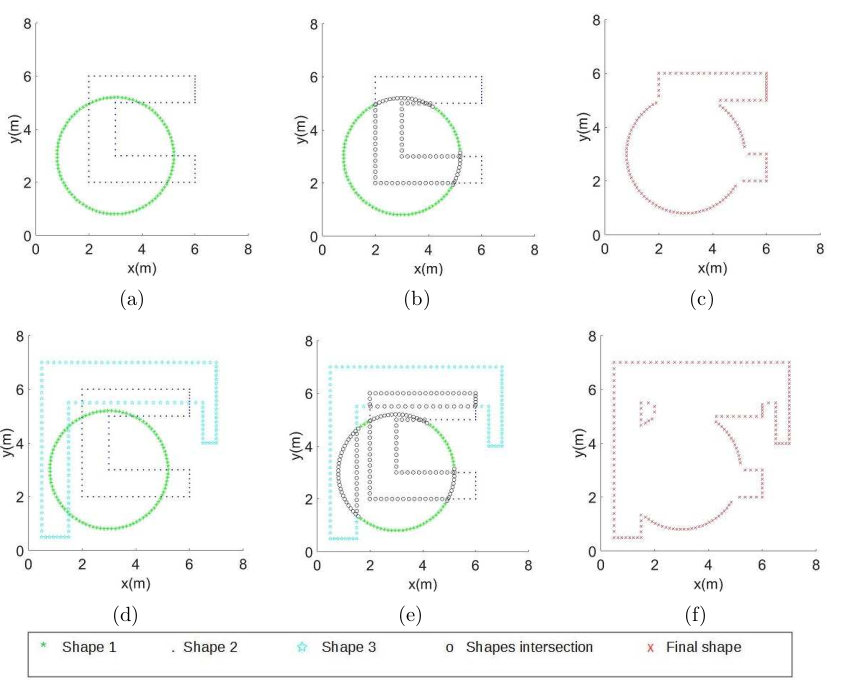
\includegraphics[scale=0.4]{assets/3_7.png}
    \caption{Frontier points processing wile assuming two concave map shapes in the first line and three in the second line. (a) and (d) represent two and three convex map shapes, respectively; (b) and (e) represent the frontier points in overlap (intersection); and (c) and (f) represent the obtained frontier points after processing (final shape).}
    \label{fig:3.7}
\end{figure}
Results show that only the frontier points within overlapping areas are removed. Even if some ambiguous frontier points are located within/inside the global shape – which can be confusing –, they are not deleted. This algorithm, assuming concave shapes, performs better than the previous one that assumes convex shapes. Hence, for the frontier processing, the shape of local maps are assumed concave.
\subsubsection{Utility function}
The proposed utility function in Eq. \ref{eq:3.2} aims to simultaneously increase the explored area rate and to reduce the distance of each UAV to its corresponding target. The function also considers the average of distances between each robot in the group and this target in order to maximize distances among robots.
\begin{equation}
    \mathbf{U}(UAV_i,t_j)=\mathbf{I}(t_j)exp(-\lambda.(dmin(\mathbf{P}_i,\mathbf{t}_j)+\frac{n_c-1}{d_{tot}})),
\end{equation}
where UAV i is the considered robot, $\mathbf{t}_j \in \mathcal{G}$ and $\mathbf{I}(\mathbf{t}_j)$ are respectively the candidate target and its corresponding information gain, $\lambda \in [0,1]$ is a trade-off parameter, $n_c$ is the number of UAVs in the cluster $\mathcal{C}$, and $d_{tot} = \sum_{k=1, k\neq i}^{n_c}(dmin(\mathbf{P}_k),\mathbf{t}_j) $ is the sum of the minimum distance from UAV$_k$'s pose $\mathbf{P}_k$ to the candidate target $j$. The proposed utility function is inspired from \cite{heng2015efficient} and it has been presented in our works \cite{mahdoui2017cooperative},\cite{mahdoui2018cooperative}. This function performs a trade-off between rapid exploration and a precise filling the map using a tuning parameter $\lambda$. From Figure \ref{fig:3.8}, we can notice that the larger $\lambda$, the less important the distance $d_{tot}$. Thus, a precise filling is favored over rapid exploration and vice versa.\\\\
Regarding the Multi-UAV case, the utility function is based on the average of neighbors distances. As shown in Figure \ref{fig:3.8}, with an information gain of $\mathbf{I}(\mathbf{t}_j)=25$ and three UAVs in the cluster $(n_c=3)$; an increasing distance of UAV to the target will reduce the utility function. Whereas, the larger the average distance from other UAVs w.r.t. to the target, the more the utility. So the function tends to choose the closest target to the considered UAV; but at the same time, the farthest one from the others.\\\\
In the case of a single UAV, the utility function (See Eq. \ref{fig:3.3}) tends to choose the closest target with the maximum of information gain:
\begin{equation}
    \mathbf{U}(UAV_i,\mathbf{t}_j)=\mathbf{I}(\mathbf{t}_j)exp(-\lambda.(dmin(\mathbf{P}_j,\mathbf{t}_j))),
\end{equation}
The parameter $d_{tot} = \sum_{k=1, k\neq i}^{n_c}(dmin(\mathbf{P}_k,\mathbf{t}_j)) $ represents the sum of the minimum distance between the target $\mathbf{t}_j$ and the neighbors’ poses $\mathbf{P}_k$ with $k \in [1..n_c]\setminus i$. So, if $\mathbf{t}_j$ has neighboring UAVs that are too far, the utility function will increase, so t j is more likely to be chosen.\\\\
The aim in the utility function is to maximize $d_{tot}$ . We distinguish two cases where $d_{tot}$ can be too close to zero or equal to it:
\begin{figure}[H]
    \centering
    \begin{subfigure}[H]{0.4\linewidth}
        \centering
        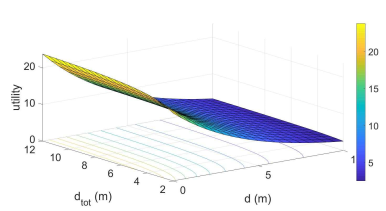
\includegraphics[width=\linewidth]{assets/3_8_a.png}
        \caption{{$\lambda=0.2$}}
        \label{fig:3.8a}
    \end{subfigure}
    \begin{subfigure}[H]{0.4\linewidth}
        \centering
        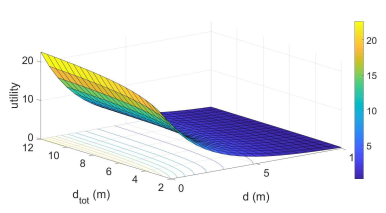
\includegraphics[width=\linewidth]{assets/3_8_b.png}
        \caption{{$\lambda=0.4$}}
        \label{fig:3.8b}
    \end{subfigure}
    \begin{subfigure}[H]{0.4\linewidth}
        \centering
        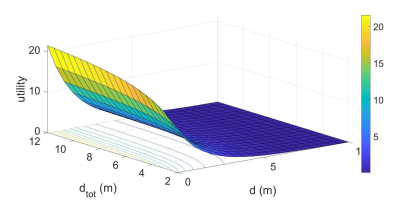
\includegraphics[width=\linewidth]{assets/3_8_c.png}
        \caption{{$\lambda=0.6$}}
        \label{fig:3.8c}
    \end{subfigure}
    \begin{subfigure}[H]{0.4\linewidth}
        \centering
        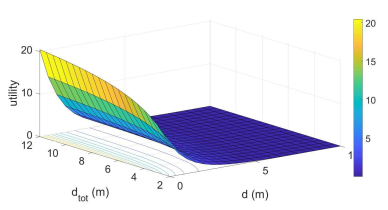
\includegraphics[width=\linewidth]{assets/3_8_d.png}
        \caption{{$\lambda=0.8$}}
        \label{fig:3.8d}
    \end{subfigure}
    \caption{{Utility function behavior: $\mathbf{I}(t_j)=25, n_c=3, d_{tot} = \sum_{k=1, k\neq i}^{n_c}(dmin(\mathbf{P}_k,\mathbf{t}_j))$. The average distance of other UAVs $d_{tot}$ has a minimum value different from zero since $n_c$ is different from zero too.}}
    \label{fig:3.8}
\end{figure}
\begin{itemize}
    \item There are no neighbors. In this case, there is one UAV in the fleet: $n_c=1$. The utility function in Eq. \ref{eq:3.3} is used.
    \item The candidate target $\mathbf{t}_j$ and the neighbors’ poses $\mathbf{P}_k$ with $k \in [1..n_c]\setminus i$ are almost confused (too close to each others). In this case $\mathbf{t}_j$ is less likely to be chosen.
\end{itemize}
Yet, this parameter $d_{tot}$ could have a high value when:
\begin{itemize}
    \item There is one UAV too far from $\mathbf{t}_j$.
    \item There are several UAVs with relatively short distance from $\mathbf{t}_j$.
\end{itemize}
So, in order to avoid these ambiguous situations, the average of $d_{tot}$ is considered by using $\frac{n_c}{d_{tot}}$.
\subsection{Goal assignment process}
In order to make appropriate UAV-to-target assignment, the utility of reaching each candidate frontier is considered. The goal assignment process is described in Algo. \ref{alg:3.5}.\\\\
For each UAV$_i$ , the utilities of reaching all the candidate targets are computed. The target $\mathbf{t}_g$ that maximizes the utility is computed and, the assignment $\theta(UAV_i,\mathbf{t}_g)$ is performed. Then, the remaining candidate targets $\mathcal{G}\setminus \mathcal{T}$ are scheduled in order to avoid to select a target too close to $\mathbf{t}_g$ , in the next iteration. Also, $\mathbf{t}_g$ is removed from $\mathcal{G}$ to prevent from assigning the same target to different robots. This assignment process is performed for the available UAVs in $\mathcal{C}$ in a sequential manner until getting all assigned targets $\mathbf{t}_g \in \mathcal{T}$ with $g \in [1..n_t]$ (See Figure \ref{fig:3.2})
\begin{algorithm}[H]
    \caption{Goal assignment algorithm.}
    \label{alg:3.5}
    \hspace*{\algorithmicindent} \textbf{Input:} {Candidate targets $\mathbf{t}_k \in \mathcal{G}, k \in [1..n_g]$ and their respective information gain $\mathbf{U}(\mathbf{t}_k)$, poses $\mathbf{P}_i$ of all robots in the considered cluster $\mathcal{C}$.}\\
    \hspace*{\algorithmicindent} \textbf{Output:} {$\theta(UAV_i,\mathbf{t}_g)$ assignment of UAV$_i$ with target $g$.}
    \begin{algorithmic}[1]
        \STATE $\mathcal{T}=\theta$
        \WHILE{no goal for UAV$_i$}
        \STATE Compute its corresponding utility of reaching each remaining candidate goal $\mathbf{U}(UAV_i,\mathbf{t}_k)$ with $\mathbf{t}_k \in \mathcal{G}\setminus \mathcal{T}$.
        \STATE $t_g=argmax_{t_k \in \mathcal{G}\setminus \mathcal{T}}(\mathbf{U}(UAV_i,\mathbf{t}_k))$.
        \STATE Schedule the information gain of the remaining candidates $\mathbf{t}_k \in \mathcal{G} \setminus \mathcal{T}$.
        \STATE $\mathcal{T}=\mathcal{T}\cup t_g$.
        \ENDWHILE
        \RETURN $\theta(UAV_i, \mathbf{t}_g)$ assignment.
    \end{algorithmic}
\end{algorithm}
\subsubsection{Stop condition}
The goal selection process is realized by each cluster/group-\textit{leader} (if $n>n-c$ ) or the Fleet- \textit{leader} (if $n=n_c$). This assignment aims to, cooperatively, distribute the robots in the environment to explore simultaneously different unknown regions. As long as candidate frontier points are still available, the \textit{leader} continues to assign targets to \textit{explorers} and they attempt to reach their assigned goals. When the \textit{leader} notices that no candidate targets are left, that means that all the environment has been explored successfully and the mission is accomplished. Thus, it has to send back to the \textit{explorers} an acknowledgment to prevent them assuming a communication loss.
\subsubsection{Loop rate}
The target assignment process is performed at each loop. The frequency of assigning targets impacts the duration and the efficiency of the mission. In a distributed approach, as soon as the UAV reaches its current target, it selects a new one without consulting the others. In a centralized approach, the first UAV to reach its current target has to wait until the others reach their respective targets. This can be a problem as soon as one of them fails or leaves the mission. Another possibility is to begin to assign targets once one UAV reaches its target. But this may generate incomplete tasks. In the proposed strategy, the frequency of assignment or loop rate $r$ is predefined depending on the average of time to reach a target (See Eq. \ref{eq:3.4}).
\begin{equation} \label{eq:3.4}
    r \in [\frac{s}{v_{i,max}},\frac{s}{v_{i,min}}]
\end{equation}
where $s$ is the maximum sensor range and $v_i$ is the UAV's velocity.
\subsubsection{Scheduling the information gain}
The information gain of each remaining candidate target $\mathbf{I}(\mathbf{t}_k)_{t-1}$ at time $t-1$ with $\mathbf{t}_k \in \mathcal{G} \setminus \{t_g\}$, that belongs to the threshold range $[r_{min} , r_{max} ]$, is scheduled at time $t$ depending on its distance w.r.t. the target $t_g$ , using Eq. \ref{eq:3.5}. Figure \ref{fig:3.9} represents an example of the function shape used to schedule the information gain. The example shows a Gaussian function with an amplitude that corresponds to the information gain maximum value; a center that corresponds to the target position $(\mathbf{t}_g(x), \mathbf{t}_g(y))$; and $\sigma_x$ and $\sigma_y$ that spread the blob in $x$ and $y$ axis, respectively.
\begin{figure}[H]
    \centering
    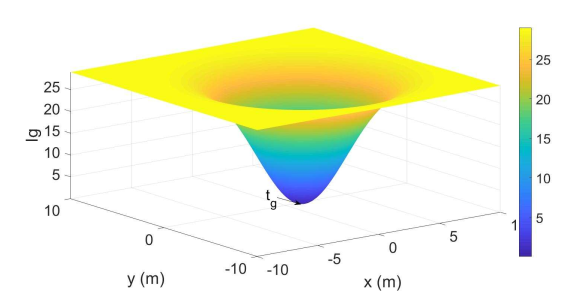
\includegraphics[scale=0.6]{assets/3_9.png}
    \caption{Example of the shape function to schedule the information gain($\mathbf{I}(\mathbf{t}_k)_{t-1}=29,(\mathbf{t}_g(x),\mathbf{t}_g(y))=(1.25,-0.275), \sigma_x=\sigma_y=3$).}
    \label{fig:3.9}
\end{figure}
\begin{equation}\label{eq:3.5}
    \mathbf{I}(\mathbf{t}_k)_t=\mathbf{I}(\mathbf{t}_k)_{t-1}(1-exp(-(\frac{(\mathbf{t}_k(x)-\mathbf{t}_g(x))^2}{2.\sigma_x^2}+\frac{(\mathbf{t}_k(y)-\mathbf{t}_g(y))^2}{2.\sigma_y^2}))),
\end{equation}
where $\mathbf{t}_k(x)$ and $\mathbf{t}_k(y)$ are the remaining candidate target coordinates; $\mathbf{t}_g(x)$ and $\mathbf{t}_g(y)$ are the target coordinates; and $\sigma_x$ and $\sigma_y$ are the spreads of the blob. The smaller the distance of the frontier point $\mathbf{t}_k$ w.r.t. the target $\mathbf{t}_g$, the smaller the information gain. When reducing the information gain, the candidate targets are less likely to be chosen and thus, robots ensure a certain distance among their future targets.
\subsection{Path planning and control}
As explained in Section 5.2 of Chapter 1, UAVs are assumed to navigate in a simplified 2D environment with a fixed $z$ value. Block \textbf{6} in Figure 1.6 is responsible for planning a path to the selected target and attempting to reach it. These tasks are ensured by the \textit{move} base\footnote{Source: \url{http://wiki.ros.org/move_base}} package.\\\\
For the navigation task, each UAV maintains a local and a global planner along with a local and a global costmap, respectively. The costmap is a 2D cell grid $\mathcal{L}$ with additional inflation that consists in propagating cost values out from occupied cells and decreasing them with distance. The global costmap has the size of the UAV’s map whereas, the local costmap has a fixed size moving window. Given a starting point – the current pose – and an endpoint – the assigned target – in the global costmap, the global planner produces a plan using a navigation function computed with Dijkstra algorithm \cite{dijkstra1959note}. It consists in following the adjacent free cells until reaching the goal. Then taking into account the local costmap, the local planner generates velocity commands for the UAV’s mobile base. A recovery rotational behavior is also performed when needed in order to clear the robot’s field of view.\\\\
The target assigned by the \textit{leader} is ensured to belong to an unknown area using the exploration strategy. The trajectory planning process is performed locally on each robot. And since the UAVs do not exchange their local maps nor fuse them, they are likely to revisit already explored areas while following the planned path. To minimize these overlapped regions during navigation, a priority is given to frontier points $\mathbf{f}_{i,j}$ to be a target for UAV$_i$ over UAV$_k$ with $k \neq i$. This helps the UAV to maintain the same direction during exploration. The \textit{move} base package is a 2D navigation stack. However, to avoid drifting on the $z$ axis, a control command is added to keep a static $z$ altitude (See Figure \ref{fig:3.10}).
\begin{figure}[H]
    \centering
    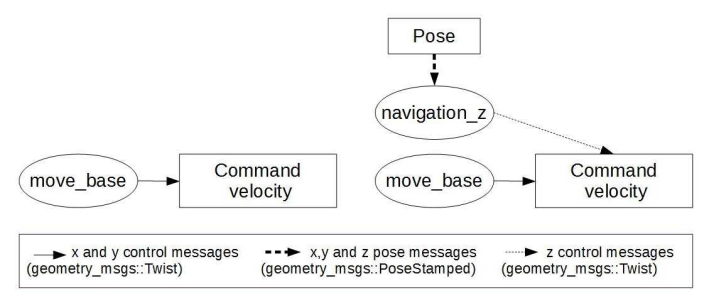
\includegraphics[scale=0.4]{assets/3_10.png}
    \caption{From 2D (left) to 3D (right) navigation stack. The \textit{navigation} z is a ROS process developed to provide a control command on the z axis.}
    \label{fig:3.10}
\end{figure}
\section{Result and discussions}
Simulations have been performed to evaluate the proposed exploration strategy. Additional tests while using relative localization have been done to measure the system performances. The simulations are performed using Robot Operating System (ROS) running on a 2.60GHz i7 Linux machine. For the quad-rotor simulation, the AR-drone model\footnote{Source: \url{http://wiki.ros.org/ardrone_autonomy}} equipped with an RGB-D camera in a forward-looking configuration, is used. A bounded unknown environment is generated using \textit{Gazebo} simulator. The number of robots used for evaluation is limited to three, however, the proposed system architecture is not constrained to a fixed number of robots.
\subsection{Parameters tuning}
For an effective evaluation of the exploration strategy, we run some tests to set the most adequate parameters configuration.
\subsubsection{Trade-off parameter $\lambda$}
The utility function (See Eq. \ref{eq:3.2}) used in the exploration strategy can be tuned, using a trade off parameter $\lambda$, between fast exploration and filling in details the map.\\\\
Figure \ref{fig:3.11} shows different runs while varying this parameter. By increasing $\lambda$, the information gained when reaching the goal is favored over the distance and thus, the cost to it, and vice versa. So, when $\lambda$ is small, the traveled distance is small and so the exploration time. Though, some times during the mission, high values of $\lambda$ are noticed to reach higher exploration rate than smaller ones.
\begin{figure}[H]
    \centering
    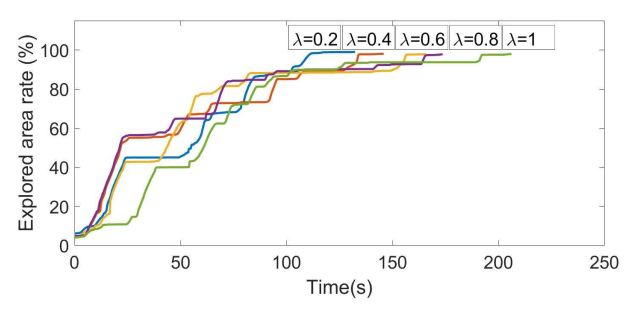
\includegraphics[scale=0.5]{assets/3_11.png}
    \caption{The impact of varying the trade off parameter $\lambda$ over exploration itme.}
    \label{fig:3.11}
\end{figure}
\subsubsection{Loop rate $r$}
The frequency or loop rate $r$ of target assignment may also affect exploration time performance. The values of $r$ vary to take into account the robot velocity $\mathbf{v}_i$ and the sensor’s maximum range $s$. The impact of varying the loop rate is evaluated in Figure \ref{fig:3.12}.
\begin{figure}[H]
    \centering
    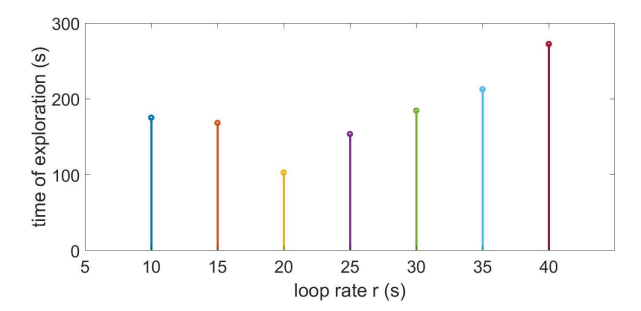
\includegraphics[scale=0.5]{assets/3_12.png}
    \caption{Exploration time while varying the loop rate $r$.}
    \label{fig:3.12}
\end{figure}
Given a robot velocity $\mathbf{v}_i=\{0.1,0.3\}m.s^{-1}$ and a maximum sensor range $s=4m$, the loop rate variates in $r \in [10,40]$. This parameter should not be too small to allow the robot to reach its target; nor too big to prevent long waiting times for the next goal assignment.
\subsubsection{Common parameters}
Depending on results in Figure \ref{fig:3.11} and Figure \ref{fig:3.12}, respectively, $\lambda$ is set to $0.2$ and $r$ to $20s$ in order to maximize the explored area rate while minimizing the mission time. The simulation parameters are summarized in Table \ref{tab:3.1}.
\begin{table}[H]
    \centering
    \caption{Common parameters.}
    \label{tab:3.1}
    \begin{tabular}{|l|l|}\hline
        \makebox[5em]{\textbf{Parameter}}                  & \makebox[5em]{\textbf{Value}}
        \\\hline
        RGB-D horizental FoV                               & $\pi/ 3$                      \\\hline
        Trade-off parameter $\lambda$                      & 0.2                           \\\hline
        RGB-D maximum range $s (m)$                        & 4                             \\\hline
        Min distance among frontiers $d (m)$               & 0.3                           \\\hline
        Occupancy grid resolution $(m)$                    & 0.05                          \\\hline
        Range to schedule the $\lg[\sigma_x,\sigma_y] (m)$ & $[3,3]$                       \\\hline
        Loop rate $l (s)$                                  & 20                            \\\hline
        Enviroment dimension $(m^2)$                       & $8 \times 8$                  \\\hline
        Linear velocity $v_i (m.s^{-1})$                   & $[0.1,0.3]$                   \\\hline
        Angular velocity $w_i (rad.s^{-1})$                & $[0.1,0.3]$                   \\\hline
    \end{tabular}
\end{table}
\subsection{Exploration strategy performances}
The proposed exploration strategy has been evaluated in terms of distribution of the robots in the environment, overlap rate, exploration time, and total traveled distance by each robot.
\subsubsection{Maps evolution during the mission}
While reaching their respective assigned goals, each robot is in charge of creating a detailed grid map of the visited area in order to get a global map of the environment. Figure \ref{fig:3.13} illustrates the growth of the reconstructed 3D occupancy grid map at different times during the mission. Note that to reach $99\%$ of coverage, a lot of time is spent.\\\\
Figure \ref{fig:3.14} shows the evolution of the respective projected 2D local grid map of two robots during a cooperative exploration mission. The global projected 2D grid map is also created and represented for evaluation (the occupancy grid matching process introduced in Algorithm 2.1 in Chapter 2 is used). The robots’ initial positions are $(1,0,0)$ for UAV$_1$ and $(1,-3,0)$ for UAV$_2$. Despite a relatively close initial position, the proposed strategy effectively spreads the robots so that UAV$_1$ is in charge of the left side of the environment and UAV$_2$ of the right one.
\subsubsection{Frontier points evolution during the mission}
The target is chosen from the candidate frontier points that define the edges of an environment not previously explored. These candidates are selected from the final frontier points of each UAV in the fleet (See Figure \ref{fig:3.15}). During the exploration mission, the local map size increases, which leads to an increasing number of local frontier points. At the beginning of the exploration, the number of candidate frontier points increases, but as soon as the exploration evolves in time, their number decreases. At the end of the mission, when all the environment is explored, no candidate frontier points should be left.
\subsubsection{UAV's trajectories during the mission}
Figure \ref{fig:3.16} shows the explored map with the trajectories using one, two and three UAVs. The UAVs try to explore the full environment while avoiding already explored areas. In a cooperative way, each UAV is in charge of visiting an area by reaching a target that belongs to a non-explored environment. These targets are assigned by the \textit{Leader} which, even if the initial poses of the UAVs are relatively close, effectively spreads them into unknown areas. The global map is composed of the superposition of all UAVs’ local maps.
\begin{figure}[H]
    \centering
    \begin{subfigure}[H]{0.3\linewidth}
        \centering
        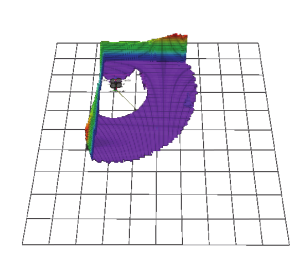
\includegraphics[width=\linewidth]{assets/3_13_a.png}
        \caption{{$3\%$ rate $(5s).$}}
        \label{fig:3.13a}
    \end{subfigure}
    \begin{subfigure}[H]{0.3\linewidth}
        \centering
        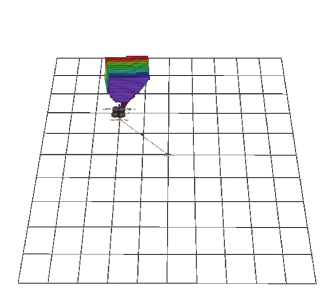
\includegraphics[width=\linewidth]{assets/3_13_b.png}
        \caption{{$20\%$ rate $(28s).$}}
        \label{fig:3.13b}
    \end{subfigure}
    \begin{subfigure}[H]{0.3\linewidth}
        \centering
        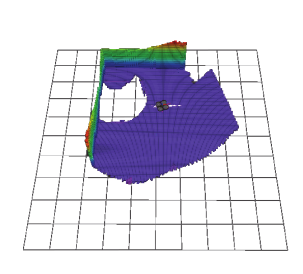
\includegraphics[width=\linewidth]{assets/3_13_c.png}
        \caption{{$31\%$ rate $(50s).$}}
        \label{fig:3.13c}
    \end{subfigure}
    \begin{subfigure}[H]{0.3\linewidth}
        \centering
        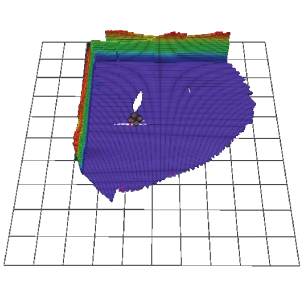
\includegraphics[width=\linewidth]{assets/3_13_d.png}
        \caption{{$40\%$ rate $(69s).$}}
        \label{fig:3.13d}
    \end{subfigure}
    \begin{subfigure}[H]{0.3\linewidth}
        \centering
        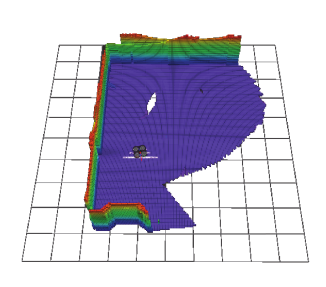
\includegraphics[width=\linewidth]{assets/3_13_e.png}
        \caption{{$50\%$ rate $(75s).$}}
        \label{fig:3.13e}
    \end{subfigure}
    \begin{subfigure}[H]{0.3\linewidth}
        \centering
        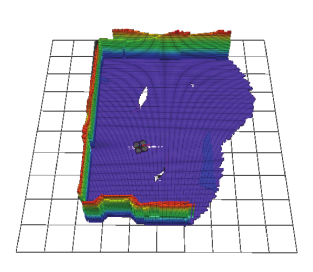
\includegraphics[width=\linewidth]{assets/3_13_f.png}
        \caption{{$60\%$ rate $(83s).$}}
        \label{fig:3.13f}
    \end{subfigure}
    \begin{subfigure}[H]{0.3\linewidth}
        \centering
        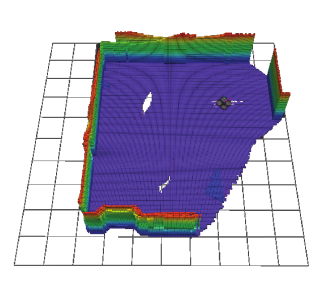
\includegraphics[width=\linewidth]{assets/3_13_g.png}
        \caption{{$70\%$ rate $(98s).$}}
        \label{fig:3.13g}
    \end{subfigure}
    \begin{subfigure}[H]{0.3\linewidth}
        \centering
        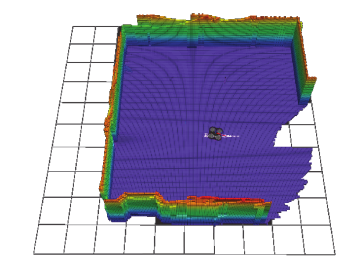
\includegraphics[width=\linewidth]{assets/3_13_h.png}
        \caption{{$81\%$ rate $(127s).$}}
        \label{fig:3.13h}
    \end{subfigure}
    \begin{subfigure}[H]{0.3\linewidth}
        \centering
        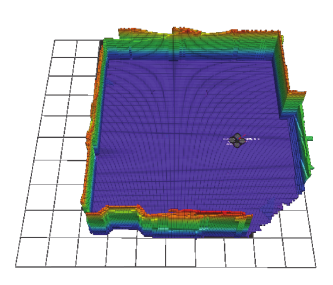
\includegraphics[width=\linewidth]{assets/3_13_i.png}
        \caption{{$90\%$ rate $(133s).$}}
        \label{fig:3.13i}
    \end{subfigure}
    \begin{subfigure}[H]{0.3\linewidth}
        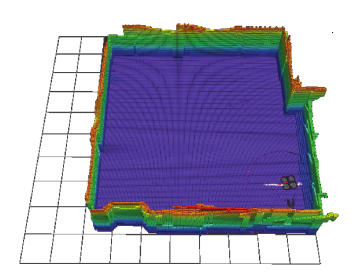
\includegraphics[width=\linewidth]{assets/3_13_j.png}
        \caption{{$99\%$ rate $(202s).$}}
        \label{fig:3.13j}
    \end{subfigure}
    \caption{Ratio of explored space during time for one UAV.}
    \label{fig:3.13}
\end{figure}
\begin{figure}[H]
    \centering
    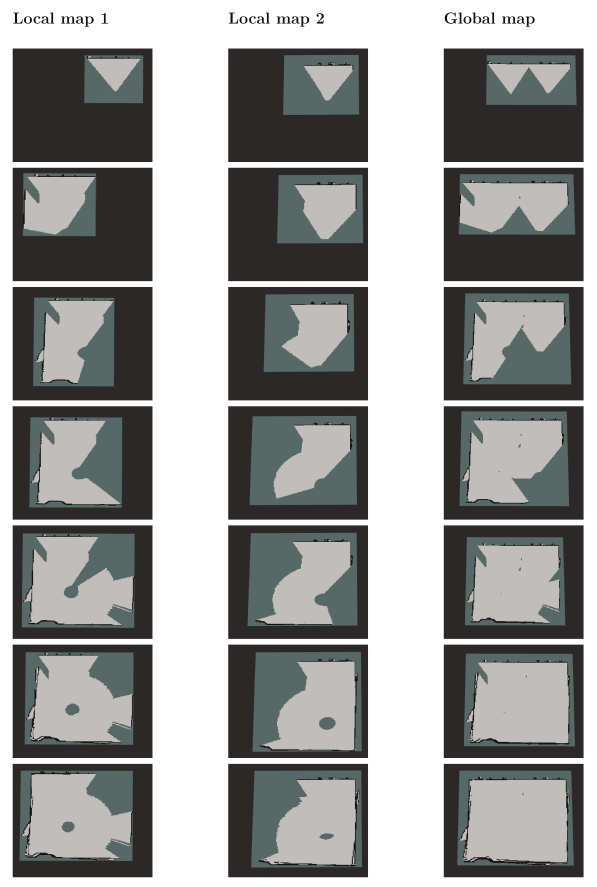
\includegraphics[scale=0.5]{assets/3_14.png}
    \caption{Coordinated exploration using two robots. Columns 1, 2 and 3 show the evolution of the local map of the UAV$_1$, the UAV$_2$ and the global map over time, respectively.}
    \label{fig:3.14}
\end{figure}
\begin{figure}[H]
    \centering
    \begin{subfigure}[H]{0.7\linewidth}
        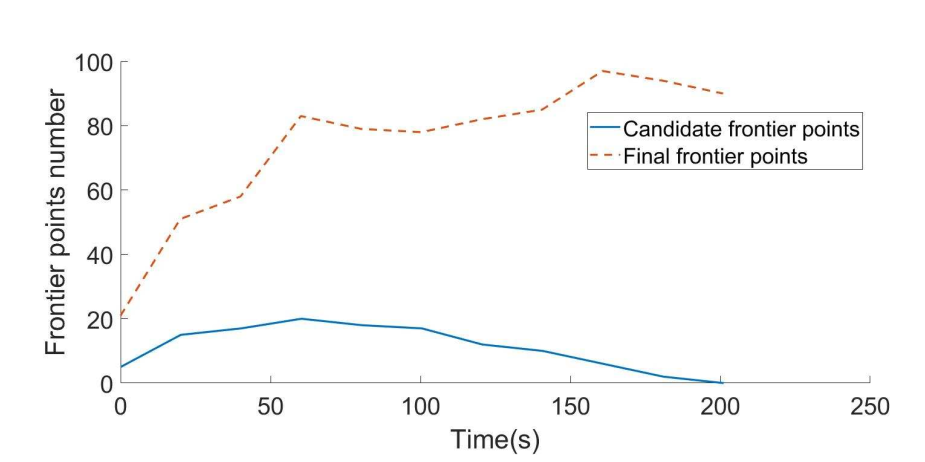
\includegraphics[width=\linewidth]{assets/3_15_a.png}
        \caption{{One UAV.}}
        \label{fig:3.15a}
    \end{subfigure}
    \begin{subfigure}[H]{0.7\linewidth}
        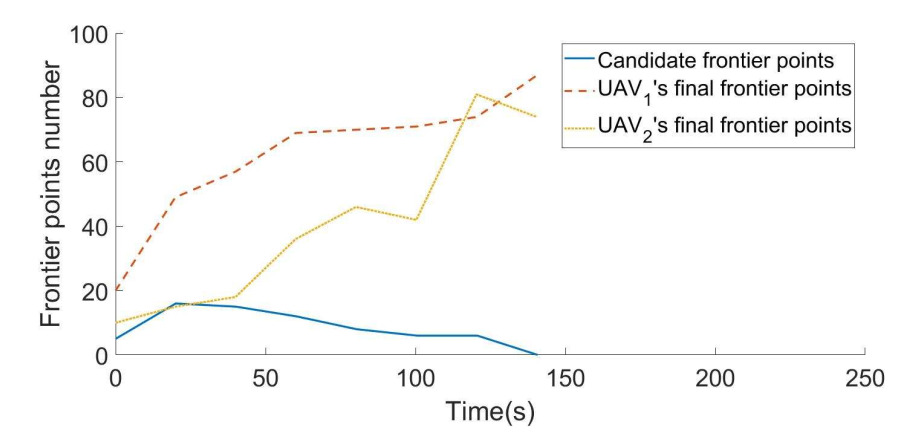
\includegraphics[width=\linewidth]{assets/3_15_b.png}
        \caption{{Two cooperative UAVs.}}
        \label{fig:3.15b}
    \end{subfigure}
    \begin{subfigure}[H]{0.7\linewidth}
        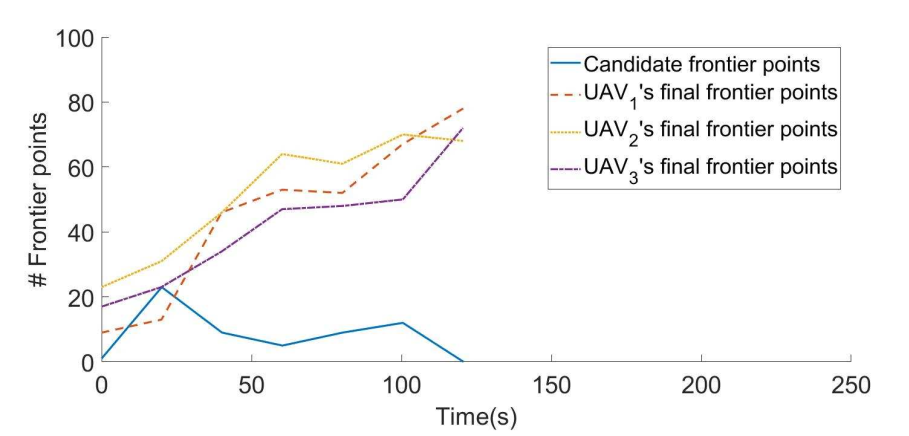
\includegraphics[width=\linewidth]{assets/3_15_c.png}
        \caption{{Three cooperative UAVs}}
        \label{fig:3.15c}
    \end{subfigure}
    \caption{The evolution of candidate and final frontier points numbers during cooperative exploration.}
    \label{fig:3.15}
\end{figure}
\begin{figure}[H]
    \centering
    \begin{subfigure}[H]{0.5\linewidth}
        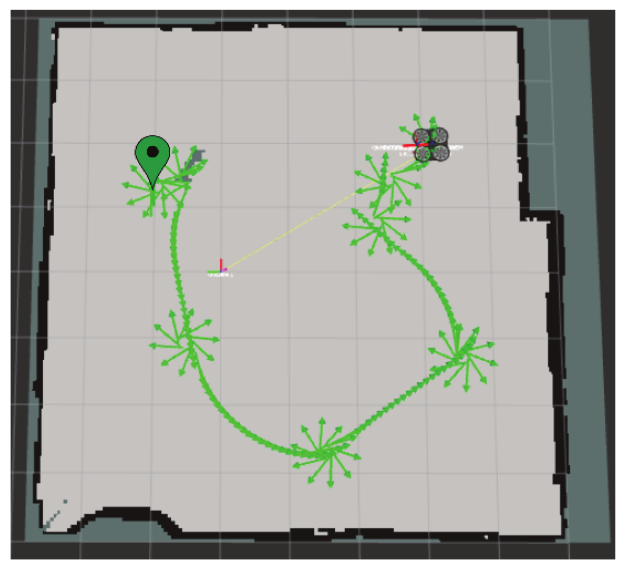
\includegraphics[width=\linewidth]{assets/3_16_a.png}
        \caption{{One UAV.}}
        \label{fig:3.16a}
    \end{subfigure}
    \begin{subfigure}[H]{0.5\linewidth}
        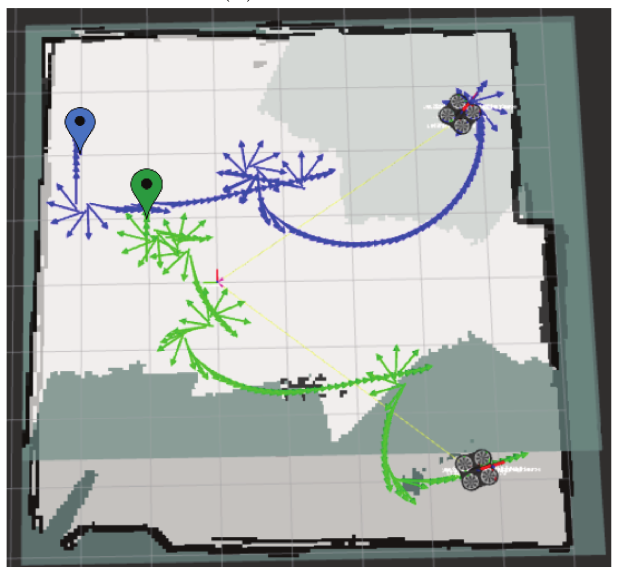
\includegraphics[width=\linewidth]{assets/3_16_b.png}
        \caption{{Two cooperative UAVs.}}
        \label{fig:3.16b}
    \end{subfigure}
    \begin{subfigure}[H]{0.5\linewidth}
        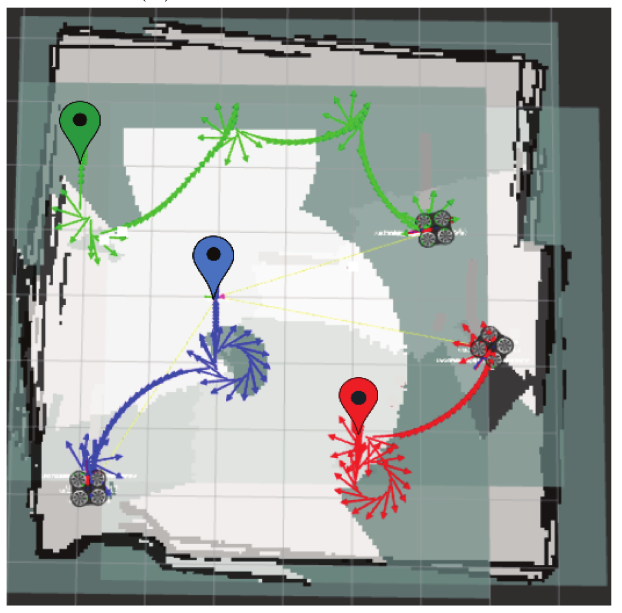
\includegraphics[width=\linewidth]{assets/3_16_c.png}
        \caption{{Three cooperative UAVs}}
        \label{fig:3.16c}
    \end{subfigure}
    \caption{Projected 2D map in a coordinated exploration with a team of one, two and three UAVs. Green, blue and red markers and arrows define, respectively, the initial position and the trajectory of UAV1, UAV2 and UAV3.}
    \label{fig:3.16}
\end{figure}
\subsubsection{Goal assignment evaluation: Distribution of the robots in the environment}
The goal assignment process is performed according to the algorithm described in Section 3.6. Nevertheless, after assigning a target to the first robot in the list, the same target or another one close to it may be assigned to the second robot in the list. To overcome these issues, the information gains of the remaining candidate targets are scheduled. This allows to discard an already assigned target and keep a certain distance between the new target and the previous one assigned.\\\\
Suppose that a target is assigned to the first robot in the cluster list. Figure \ref{fig:3.17} shows the goal selected for the second robot when a sequential assignment is performed:
\begin{itemize}
    \item Without further frontier points processing (See Figure \ref{fig:3.17b}). Consequently, the same target is assigned to two different robots.
    \item While removing the assigned target from the remaining candidate frontier points (See Figure \ref{fig:3.17c}). Consequently, the second target is relatively close to the first one assigned.
    \item While scheduling the information gain after each target assignment (See Figure \ref{fig:3.17d}). Consequently, the assigned targets are spaced out into the environment. The information gain is scheduled following Eq. \ref{eq:3.5}. The information gain value increases with distance to the candidate target $\mathbf{t}_g$.
\end{itemize}
The goal assignment process may sometimes be not optimal since it depends on the robots’ order in the list. For example, suppose that robots UAV$_i$ and UAV$_j$ have the same best target assignment t k such that it offers the maximum utility over candidate frontier points where Eq.\ref{eq:3.6} and Eq. \ref{eq:3.7} are verified.
\begin{equation}\label{eq:3.6}
    \mathbf{t}_k=argmax_{t_m}\mathbf{U}(UAV_i,\mathbf{t}_m)
\end{equation}
with $\mathbf{t}_m \in \mathcal{G}$.
\begin{equation}\label{eq:3.7}
    \mathbf{t}_k=argmax_{t_n}\mathbf{U}(UAV_j, \mathbf{t}_n)
\end{equation}
with $\mathbf{t}_n \in \mathcal{G}$.\\
UAV$_i$ have another candidate frontier point $\mathbf{t}_l$ with:
\begin{equation}\label{eq:3.8}
    \mathbf{\mathit{U}}(UAV_i, \mathbf{t}_k) > \mathbf{\mathit{U}}(UAV_i,\mathbf{t}_l) > \mathbf{\mathit{U}}(UAV_j, \mathbf{t}_k)
\end{equation}

\begin{figure}[H]
    \centering
    \begin{subfigure}[H]{0.6\linewidth}
        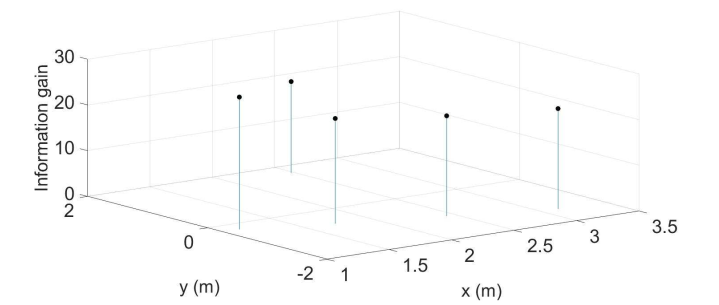
\includegraphics[width=\linewidth]{assets/3_17_a.png}
        \caption{{Candidate targets.}}
        \label{fig:3.17a}
    \end{subfigure}
    \begin{subfigure}[H]{0.6\linewidth}
        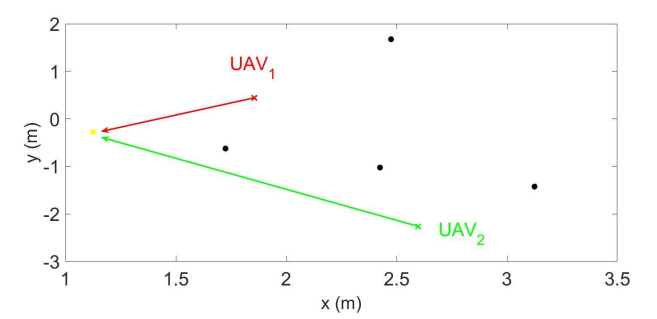
\includegraphics[width=\linewidth]{assets/3_17_b.png}
        \caption{{Case 1.}}
        \label{fig:3.17b}
    \end{subfigure}
    \begin{subfigure}[H]{0.6\linewidth}
        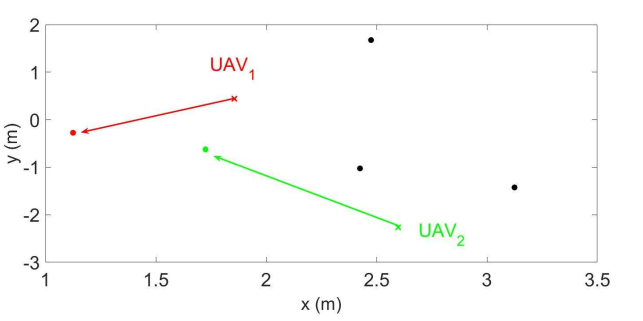
\includegraphics[width=\linewidth]{assets/3_17_c.png}
        \caption{{Case 2.}}
        \label{fig:3.17c}
    \end{subfigure}
    \begin{subfigure}[H]{0.6\linewidth}
        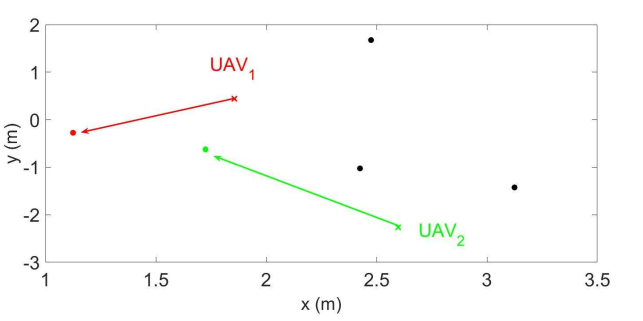
\includegraphics[width=\linewidth]{assets/3_17_c.png}
        \caption{{Case 3.}}
        \label{fig:3.17d}
    \end{subfigure}
    \caption{Goal assignment: After assigning a target to UAV$_1$ , a target is assigned in a sequential manner to UAV$_2$ . (a) represents the candidate frontier points with their respective information gain. (b), (c), and (d) represent, respectively, the targets assignment when: No further process is performed for the remaining candidate targets; UAV$_1$ ’s target is removed from the remaining candidate targets and; the information gain of the remained candidate targets are scheduled.}
    \label{fig:3.17}
\end{figure}
So the optimal solution would be to assign $\mathbf{t}_l$ to UAV$_i$ and $\mathbf{t}_k$ to UAV$_j$ . But, if UAV$_i$ is the first in the list, $\mathbf{t}_k$ is assigned to it and another candidate frontier point with less utility than $\mathbf{t}_k$, is assigned to UAV$_j$. Thus, the solution with sequential goal assignment is not always optimal.\\\\
To overcome this problem, all the numbers of possible combination $\frac{n_g!}{n_g!(n_g-n_c)!}$ with $n_g$ the number of candidate targets and $n_c$ the number of robots, need to be considered. This increases considerably the computation time by increasing the number of robots. Therefore, in the proposed algorithm, sequential assignment is favored over computing all possible permutations.
\subsubsection{Explored space rate evaluation}
This evaluation aims at quantifying the amount of explored spaces during the mission. Figure \ref{fig:3.18} shows the explored space rate performed by each UAV in the fleet. The more UAVs in the environment, the less the exploration rate demanded by each one. A robot has no need to continue exploring an area if it has already been explored by another one. Thus, the mission time is considerably reduced.
\subsubsection{Overlap rate evaluation}
The use of an effective goal assignment process should limit the generated overlap. In Figure \ref{fig:3.19}, the time evolution of overlap is evaluated using two cooperative robots. The overlap undergoes a significant increase at the end of the exploration to reach $33\%$. This is explained by the closeness of the local maps at the end of the mission to precisely fill the global grid map.
\begin{figure}[H]
    \centering
    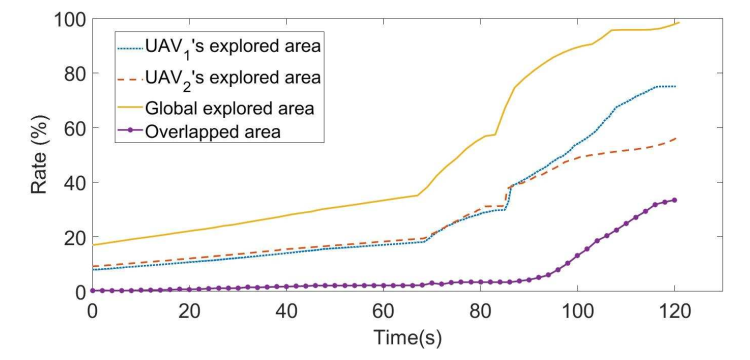
\includegraphics[scale=0.4]{assets/3_19.png}
    \caption{Explored and overlapped area rate using two cooperative UAVs.}
    \label{fig:3.19}
\end{figure}
\subsubsection{Traveled distance evaluation}
To effectively evaluate the exploration strategy performance in terms of distance traveled by each UAV, different runs with one, two and three UAVs have been conducted where explored area rate reaches almost $99\%$. Figure \ref{fig:3.20} shows the distance traveled by each UAV in the fleet during the mission.
\begin{figure}[H]
    \centering
    \begin{subfigure}[H]{0.7\linewidth}
        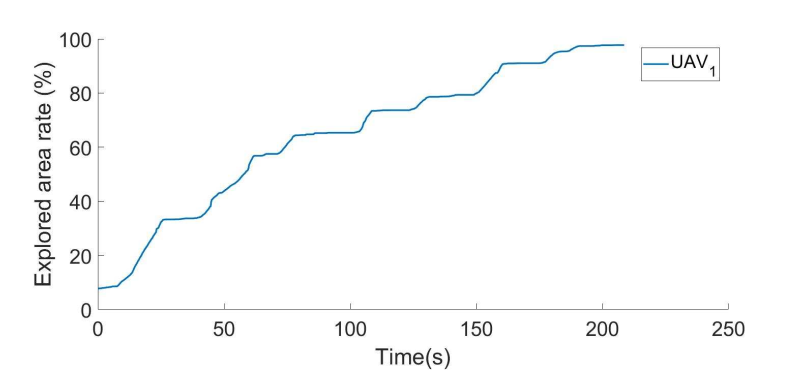
\includegraphics[width=\linewidth]{assets/3_18_a.png}
        \caption{{One UAV.}}
        \label{fig:3.18a}
    \end{subfigure}
    \begin{subfigure}[H]{0.7\linewidth}
        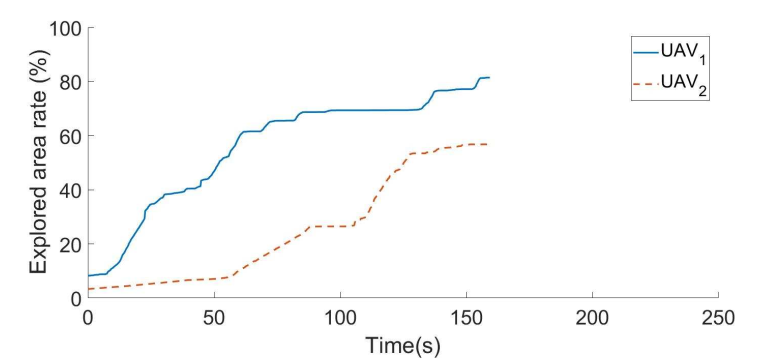
\includegraphics[width=\linewidth]{assets/3_18_b.png}
        \caption{{Two cooperative UAVs.}}
        \label{fig:3.18b}
    \end{subfigure}
    \begin{subfigure}[H]{0.7\linewidth}
        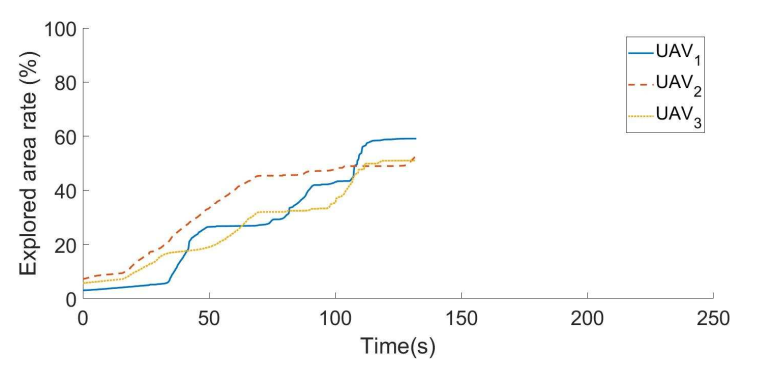
\includegraphics[width=\linewidth]{assets/3_18_c.png}
        \caption{{Three cooperative UAVs}}
        \label{fig:3.18c}
    \end{subfigure}
    \caption{Explored space rate with one, two and three UAVs.}
    \label{fig:3.18}
\end{figure}
\begin{figure}[H]
    \centering
    \begin{subfigure}[H]{0.7\linewidth}
        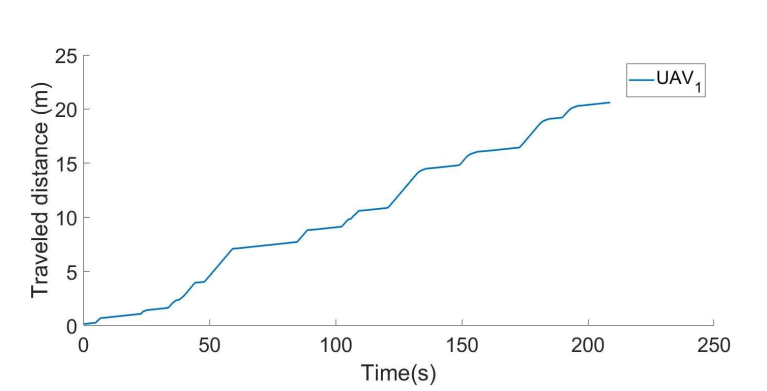
\includegraphics[width=\linewidth]{assets/3_20_a.png}
        \caption{{One UAV.}}
        \label{fig:3.20a}
    \end{subfigure}
    \begin{subfigure}[H]{0.7\linewidth}
        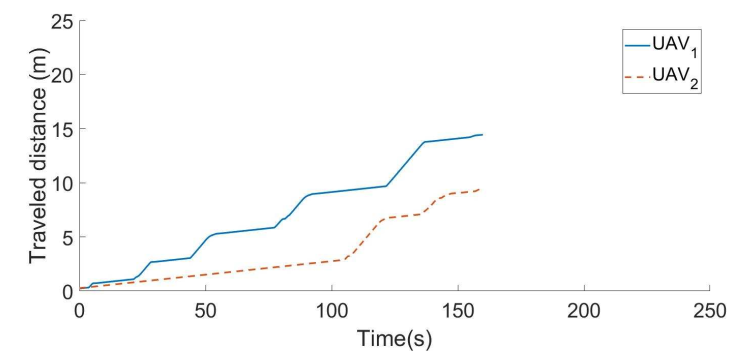
\includegraphics[width=\linewidth]{assets/3_20_b.png}
        \caption{{Two cooperative UAVs.}}
        \label{fig:3.20b}
    \end{subfigure}
    \begin{subfigure}[H]{0.7\linewidth}
        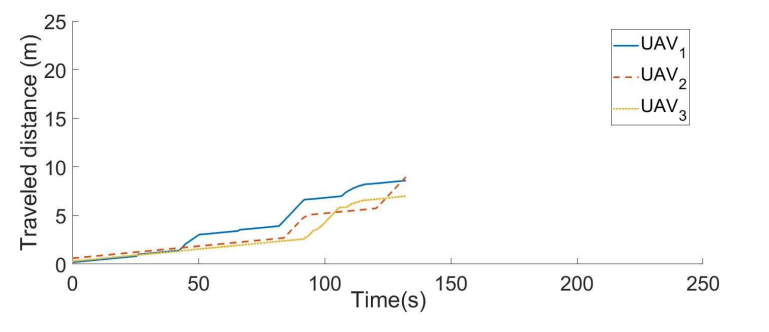
\includegraphics[width=\linewidth]{assets/3_20_c.png}
        \caption{{Three cooperative UAVs}}
        \label{fig:3.20c}
    \end{subfigure}
    \caption{Traveled distance by each UAV with one, two and three cooperative UAVs.}
    \label{fig:3.20}
\end{figure}
The distances traveled by each UAV using one, two and three UAVs in the fleet are compared in Figure \ref{fig:3.21}. This distance decreases with the number of UAVs. The average distance traveled by each UAV is reduced by $55\%$ for 2 UAVs and by $62\%$ for 3 UAVs. The error of the traveled distance is slightly reduced from one to two and three UAVs.
\begin{figure}[H]
    \centering
    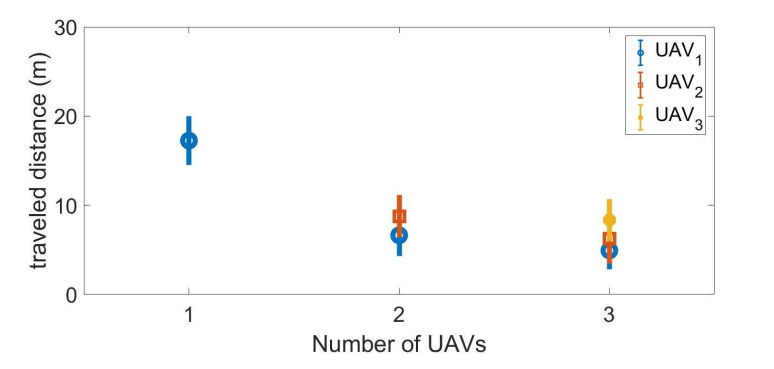
\includegraphics[scale=0.4]{assets/3_21.png}
    \caption{Traveled distance evaluation.}
    \label{fig:3.21}
\end{figure}
\subsubsection{Exploration time evaluation}
For the exploration time evaluation, different runs have been performed using 1, 2 and 3 UAVs. Figure \ref{fig:3.22} shows that the average of exploration time decreases when the number of robots in the fleet increases. The computed error decreases as well. The time is reduced by $25\%$ for 2 UAVs and by $30\%$ for 3 UAVs. The exploration time and distance are not divided by 2 or 3 when multiplying by 2 or 3 the number of robots, respectively. During these simulations, the robots’ initial positions are: $(1,0,0)$ for one UAV; $(1,0,0)$ and $(1,-3,0)$ for two UAVs; and $(1,1,0)$, $(1,-1,0)$ and $(1,-3,0)$ for three UAVs.
\begin{figure}[H]
    \centering
    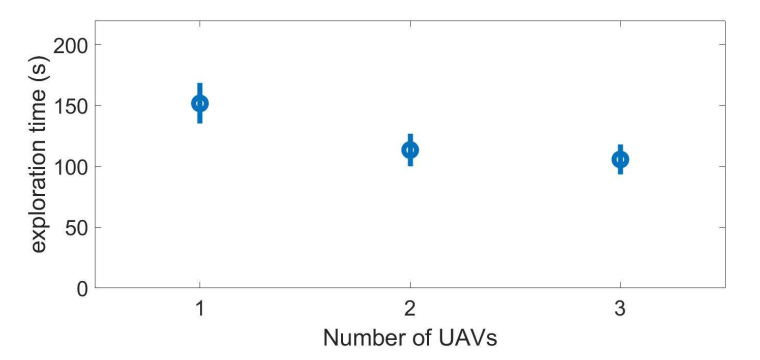
\includegraphics[scale=0.4]{assets/3_22.png}
    \caption{Average exploration time.}
    \label{fig:3.22}
\end{figure}
The results presented in Section 4.2 were evaluated without a relative localization. So, for a more challenging realistic scenario, runs with relative localization algorithm have been performed to evaluate system performances using SLAM.
\subsection{Exploration mission using relative localization algorithm}
Toward a more realistic scenario, the ORB-SLAM2 approach (introduced in Section 5 of Chapter 2) has been implemented to perform relative localization (See Figure \ref{fig:3.23}).
\begin{figure}[H]
    \centering
    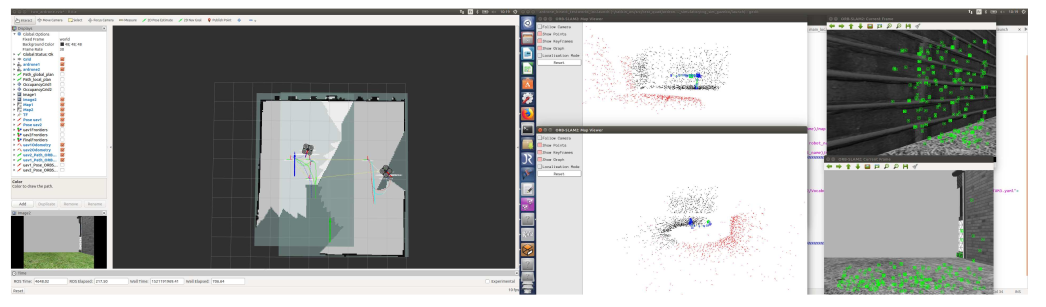
\includegraphics[scale=0.3]{assets/3_23.png}
    \caption{Two UAVs navigation using ORB-SLAM2. Rviz image (left) shows, for each UAV, the constructed 2D occupancy grid map, its estimated trajectory and the corresponding ground truth. The point cloud (middle) represent the sparse reconstruction of the environment made by each UAV. And, the green markers (right) represent the features computed by each UAV to perform localization.}
    \label{fig:3.23}
\end{figure}
Each robot performs SLAM where it constructs its map in its local reference frame $^WF_i$ , and estimates its relative pose $\mathbf{p}_i$ within it. Then, the fleet performs cooperative explo- ration using some specific information exchanged among UAVs. But, these information have to be in a common reference frame. Therefore, information such as the pose $\mathbf{p}_i$ and the frontier points $\mathbf{f}_{i,j}$ are necessarily transformed into the global reference frame $^0W$ before being exchanged. Hence, the \textit{leader} makes all the needed computation and sends back to the \textit{explorers} the targets in $^0W$. When a robot receives its assigned goal, it transforms it into $^WF_i$ to plan a path to it.\\\\
To perform a transformation from local reference $^WF_i$ to global one $^0W$, the robot has to know – at least – its initial pose w.r.t. $^0W$. As explained in Section 5.2 of Chapter 1, the global reference frame of the environment is initialized such that it coincides with the local reference frame of the first group-\textit{leader} in the fleet which is UAV$_1$ in the considered example of Equation \ref{eq:3.9}.
\begin{equation}\label{eq:3.9}
    ^0W\equiv ^WF_1,
\end{equation}
Then, by detecting this robot using tags mounted on it, the other robots are able to estimate their respective transform to it $^{F_j}\begin{bmatrix}\mathbf{R} & \mathbf{t}\end{bmatrix}_{F_1}, j \in [2..n_c]$. For simulation evaluations, the information of transform – computed while detecting the tag – are assumed to be known. Figure \ref{fig:3.24} shows the exploration rate evolution during the exploration mission while using ORB-SLAM2 as the relative localization approach. The mission time using ORB-SLAM2 is reduced by $43\%$ for 2 UAVs instead of 1 UAV.
\begin{figure}[H]
    \centering
    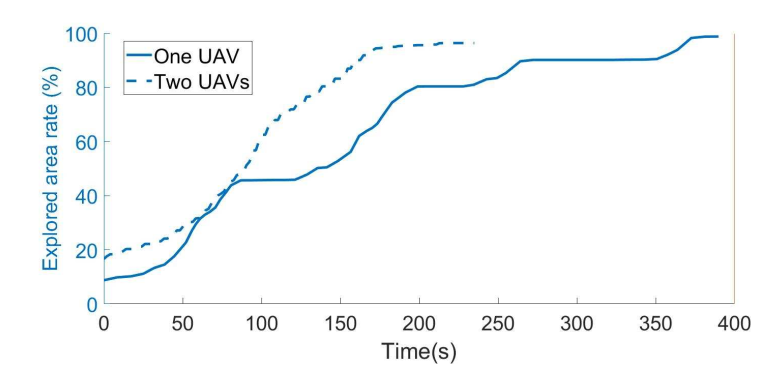
\includegraphics[scale=0.4]{assets/3_24.png}
    \caption{Explored area rate evolution during exploration mission with one and two UAVs while performing ORB-SLAM2 by each UAV.}
    \label{fig:3.24}
\end{figure}
The exploration time when using a relative localization (See Figure \ref{fig:3.24}) is relatively important compared to the exploration without SLAM (See Figure \ref{fig:3.18}) since the velocity has been considerably reduced.
\section{Conclusion}
In this chapter, we presented a state of the art of multi-robot exploration mission including the strategy used to assign a robot to a target and an utility function adopted to estimate the interest of reaching it. Then, we introduced an exploration strategy based on the group-\textit{leader} decision making. The robot-to-target assignment is performed using a novel utility function. This function makes a trade-off between fast exploration and getting a detailed grid map, and also takes into account the distance of each robot in the group from the unexplored set of targets. Also, we propose to schedule the information gain in order to efficiently spread the UAVs into the environment. Moreover, the strategy adopted exchanges the frontier points instead of a whole copy of the local map.\\\\
Results show that the proposed cooperative exploration strategy minimizes the global exploration time by $25\%$ for 2 UAVs and by $30\%$ for 3 UAVs, while minimizing the average traveled distance by each UAV by $55\%$ for 2 UAVs and by $62\%$ for 3 UAVs. Furthermore, the strategy was evaluated using a relative localization algorithm where the exploration time was reduced by $43\%$ for 2 UAVs instead of 1 UAV.
%------------------CHAPTER 4------------------------------------------------%
\chapter{Giao tiếp giữa các robot}
\section{Giới thiệu}
Một chủ đề quan trọng trong các hệ thống nhiều robot là giao tiếp giữa các robot. Tính năng này được sử dụng để điều phối và chia sẻ thông tin cụ thể. Một đội có thể được triển khai trong một số nhiệm vụ trong các khu vực tương đối khác biệt và thù địch. Tuy nhiên, những môi trường này có thể không có cơ sở hạ tầng mạng sẵn có, ngoài các liên kết truyền thông không lý tưởng.\\\\
% This chapter highlights one of the most challenging points in MRS, which is the inter- robot communication. This problem can be addressed from different perspectives; but, we have chosen to study two sub-problems, which are: network typology, and network topology and strategy for MRS robustness.
Chương này nhấn mạnh một trong những điểm thách thức nhất trong MRS, đó là giao tiếp giữa các robot. Vấn đề này có thể được giải quyết từ các quan điểm khác nhau; nhưng, chúng tôi đã lựa chọn nghiên cứu hai vấn đề nhỏ, đó là: định dạng mạng, cấu trúc liên kết mạng và chiến lược cho sự mạnh mẽ của MRS.
\section{Phân loại mạng}
% The network is used to link between different entities and to establish possible communi- cation between them. Several network types exist and can be classified in different ways.
Mạng được sử dụng để liên kết giữa các thực thể khác nhau và để thiết lập giao tiếp có thể có giữa chúng. Một số loại mạng tồn tại và có thể được phân loại theo nhiều cách khác nhau.
\subsection{Chế độ cơ sở hạ tầng so với chế độ không có cơ sở hạ tầng}
Để quản lý cơ sở hạ tầng mạng, các chế độ hiện có có thể được phân loại thành hai loại chính \cite{bekmezci2013flying},\cite{hayat2015experimental}. Loại đầu tiên là chế độ cơ sở hạ tầng, có thể được gọi là chế độ Điểm truy cập (AP) và loại thứ hai là chế độ không có cơ sở hạ tầng, gọi là Ad Hoc mode (Xem Hình \ref{fig:4.1}). Trong chế độ AP, giao tiếp UAV-to-UAV được thực hiện thông qua cơ sở hạ tầng (AP, bộ định tuyến, v.v.), không giống như chế độ Ad Hoc trong đó các nút giao tiếp trực tiếp với nhau. Chế độ Ad Hoc còn được gọi là chế độ ngang hàng. Mạng Ad Hoc có thể phát triển thành một chế độ ngang hàng khác được gọi là mạng lưới bằng cách cho phép khả năng đa bước. Thật vậy, mạng Ad-Hoc không có bất kỳ khả năng cố hữu nào cho đa bước. Các nút giao tiếp với nhau khi chúng nằm trong phạm vi giao tiếp của nhau. Trong khi đó, trong mạng lưới, các nút có thể giao tiếp trực tiếp hoặc thông qua một hoặc nhiều nút trung gian.
\begin{figure}[H]
    \centering
    \includegraphics[scale=0.4]{assets/4_1.png}
    \caption{Chế độ hạ tầng (trái) và chế độ không có hạ tầng (phải).}
    \label{fig:4.1}
\end{figure}
\begin{table}[H]
    \centering
    \caption{Chế độ cơ sở hạ tầng so với chế độ không có cơ sở hạ tầng.}
    \label{tab:4.1}
    \begin{tabular}{|l|p{4.5cm}|p{4.5cm}|}\hline
                            & \textbf{Chế độ cơ sở hạ tầng}                 & \textbf{Chế độ không có cơ sở hạ tầng}
        \\\hline
        \textbf{Ưu điểm}    & Giao tiếp đáng tin cậy                        & Kết nối trực tiếp với nhau, dễ thiết lập, mạnh mẽ với lỗi nút, cho phép mở rộng và điều chỉnh trong cấu trúc liên kết mạng. \\\hline
        \textbf{Nhược điểm} & Phần cứng đắt, phức tạp, phạm vị bị hạn chế . & Thừa trong kết nối mạng, khó bảo trì.                                                                                       \\\hline
        \textbf{Tiêu chuẩn} & 802.11                                        & 802.11, 802.15, 802.16                                                                                                      \\\hline
    \end{tabular}
\end{table}
Ban đầu, robot phải thực hiện nhiệm vụ của chúng trong môi trường không có cơ sở hạ tầng mạng. Trên thực tế, chúng trao đổi thông tin khi chúng hoạt động như một bộ định tuyến và như một AP. Vì vậy, hệ thống MRS có thể được xem như một mạng Ad Hoc di động theo quan điểm giao tiếp.
\subsection{Phân loại mạng Ad Hoc}
Mạng Ad Hoc là mạng được sử dụng phổ biến để quản lý giao tiếp đa robot. Với mạng này, mỗi robot có thể di chuyển tự do và chuyển tiếp các gói tin đến và từ mỗi robot khác tùy thuộc vào phương thức phân phối dữ liệu \cite{bouachir2014conception}. Mạng này được đặc trưng bởi chất lượng dịch vụ phức tạp, trong đó giao thức định tuyến xác định đường đi tối ưu của thông tin có tính đến sự thay đổi thường xuyên của cấu trúc liên kết. Thêm vào đó, sẽ rẻ hơn nếu nhận ra loại mạng này thay vì các loại khác (vệ tinh, di động, v.v.).\\\\
Mạng Ad Hoc có thể được phân loại thành ba loại chính là Mobile Ah doc NETwork (MANET), Vehicle Ah doc NETwork (VANET) và Flying Ad hoc NETworks (FANET). Nói chung, đối với hệ thống đa UAV, mô hình FANET được sử dụng. Bảng \ref{tab:4.2} mô tả chi tiết mỗi đặc điểm của danh mục \cite{bekmezci2013flying}, \cite{maistrenko2016experimental}, phân tích dự đoán của chúng tôi.
\begin{table}[H]
    \centering
    \caption{So sánh giữa MANET, VANET, FANET và mô hình mạng của chúng tôi.}
    \label{tab:4.2}
    \begin{tabular}{|p{2.8cm}|p{1.5cm}|p{1.5cm}|p{1.8cm}|p{1.8cm}|}\hline
        \textbf{Đặc điểm}                                                 & \textbf{MANET}                                      & \textbf{VANET}                       & \textbf{FANET}                                                                                 & \textbf{Mô hình mạng của chúng tôi}
        \\\hline
        \textbf{Tính di động}                                             & Người ở một số địa hình nhất định                   & Phương tiện ở cao tốc                & Máy bay trong kế hoạch 3D                                                                      & 3D                                  \\\hline
        \textbf{Mức độ di động}                                           & $+$                                                 & $+$                                  & $++$                                                                                           & $++$                                \\\hline
        \textbf{Chế độ di động}                                           & Điểm cách ngẫu nhiên với hướng và tốc độ ngẫu nhiên & Có khả năng dự đoán cao trên đường   & Không được xác định trước (mô hình chuyển động ngẫu nhiên của UAV, mô hình dựa trên pheromone) & Có thể dự đoán                      \\\hline
        \textbf{Thay đổi cấu trúc liên kết}                               & $+$                                                 & $+$                                  & $++$                                                                                           & $++$                                \\\hline
        \textbf{Khoảng cách giữa các nút}                                 & $+$                                                 & $+$                                  & $++$                                                                                           & $+$                                 \\\hline
        \textbf{Mật độ nút}                                               & $++$                                                & $++$                                 & $+$                                                                                            & $+$                                 \\\hline
        \textbf{Mô hình truyền thanh}                                     & Sự hiện diện hiếm hoi của đường ngắm                & Sự hiện diện hiếm hoi của đường ngắm & Sự hiện diện thường xuyên của đường ngắm                                                       & Luôn có mặt của đường ngắm          \\\hline
        \textbf{Công suất tiêu thụ và công suất tính toán thời gian sống} & $+$                                                 & $+$                                  & $++$                                                                                           & $++$                                \\\hline
        \textbf{Tiêu chuẩn}                                               & IEEE 802.11, 802.15, 802.15.4, 802.16 and 802.20    & IEEE 802.11p                         & IEEE 802.11                                                                                    & ?                                   \\\hline
    \end{tabular}
\end{table}
So sánh cho thấy FANET là mạng gần nhất với kỳ vọng của mô hình của chúng tôi. Do đó, trong số các tiêu chuẩn hiện có cho loại mạng này, IEEE 802.11b và IEEE 802.11g cung cấp tốc độ dữ liệu cao và thường được sử dụng cho các hệ thống nhiều robot.
\subsection{Phân loại cấu trúc liên kết mạng}
Cấu trúc liên kết mạng xác định điểm đầu, điểm cuối và đường dẫn của thông tin trong mạng. Đã cho các điểm mục tiêu, cấu trúc liên kết xác định tất cả các con đường có thể để đạt được chúng.\\\\
Từ quan điểm phần mềm, mạng chủ yếu có thể được phân loại theo ba cấu trúc liên kết (Xem Hình \ref{fig:4.2}\footnote{Source: From user 1983 on Wikipedia. Licensed CC BY-SA}):
\begin{figure}[H]
    \centering
    \includegraphics[scale=0.4]{assets/4_2.png}
    \caption{Mạng tập trung (trái), phi tập trung (giữa) và mạng phân tán (phải).}
    \label{fig:4.2}
\end{figure}
\begin{itemize}
    \item Mạng tập trung: Đây là cấu trúc liên kết được sử dụng nhiều nhất \cite{morgenthaler2012uavnet}, \cite{forster2013collaborative}. Tất cả các nút - còn được gọi là các trạm - được kết nối với nhau thông qua một trung tâm tập trung. Đó là khi một nút cần gửi một thông tin đến một nút khác, dữ liệu nhất thiết phải đi qua nút trung tâm để được chuyển đến đích của nó. Nếu nút trung tâm không hoạt động hoặc không thể truy cập được, không có dữ liệu nào có thể được truyền đi, điều này làm cho cấu trúc liên kết này dễ bị lỗi nút.
    \item Decentralized network: This topology is considered as a set of centralized networks connected together \cite{konolige2003map}, \cite{brand2014stereo}. One central hub is employed for every little group of nodes to send and receive the information. If a hub fails, nodes which are direactly relied to it become inaccessible.
    \item Distributed network: This topology contains nodes that are connected to each others. Unlike the centralized topology, several paths are possible to reach one destination. Also, nodes are not affected by one node's failure. This allows to increase the survivability and to decrease the vulnerability of the network. The distributed topology is attractive to ensure reliable network \cite{cunningham2010ddf}. Nevertheless, it is quite difficult to reach and to realize in reality, and the simulation are not fully distributed \cite{waharte2009coordinated}, \cite{cameron2009collaborative}, \cite{scherer2015autonomous}. This is because all processing and decision making have to be on-board the robot whichs requires an important memory and a heavy computation.
\end{itemize}
\section{Network typology}
The typology of the network represents its type and, accordingly, the characteristics introduced.
\subsection{Related work}
MRS communication is a critical problem to tackle in the robotics community. In the last decade, the great progress in wireless technologies and MRS has created a growing interest for inter-robot communication. Hence, different methods have been proposed.\\\\
To face disaster scenarios such as fire in an industrial warehouse, authors in \cite{witkowski2008ad} propose to use Wireless LAN, Bluetooth and ZigBee to form an Ad- Hoc network. Some robots of the fleet form the network infrastructure to support communication.\\\\
Authors in \cite{morgenthaler2012uavnet} use two network standards to build a multi-UAV system. A IEEE 802.11s wireless mesh network is build using UAVs carrying mesh nodes directly connected to the flight electronics. Each of these mesh nodes acts as an AP in order to form an IEEE 802.11g.\\\\
A methodology that profiles the wireless links for Linux-based networked aerial vehicles is presented in \cite{kuschnig2012profiling.} The approach includes two options to collect link quality information and to monitor the 802.11 wireless interface.\\\\
An evaluation of the standard 802.11a used between an UAV and an AP is performed in \cite{kuschnig2012profiling}. Results show that the Received Signal Strength (RSS) for the downlink decreases with the distance to the AP but remains at an acceptable level as well as the throughput.\\\\
Knowing that the visible light spectrum is much wider than the Radio Frequency spectrum, it seems interesting to uptake Visible Light Communication (VLC) based on Light Emitting Diodes (LEDs). IEEE has developed the 802.15.7 standard for short range communication using visible light. Authors in \cite{wang2014openvlc} introduce a bidirectional communication using Open VLC. This solution hardware needs a Beagle Bone Black (BBB) board and a font transceiver that employs a single LED to both transmit and receive. The solution is implemented on Linux driver that communicates directly with the LED front-end and the Linux networking stack. The main idea to reuse the same LED for both Transmitting (TX mode) and Receiving Light signal (RX mode) is that when a node is transmitting data, the other node can expect the LOW symbol of the bit 0 and makes use of this time to switch his mode from RX to TX and transmit data.\\\\
The Zigbee – based on IEEE 802.15.4 – is a protocol of high level which is particularly useful for short communication range and low consumption. Several UAVs’ application use this network \cite{asadpour2014routing}. Communication can be made under three frequency bands depending on the chipset type: 868MHz for a bit rate of 20 kbps, 915MHz for 40 kbps and 2.4GHz for 250 kbps.\\\\
Authors in \cite{vidal2015multi} adopt different sized groups composed of tactical UAVs and UAVs moving in delimited geographical areas. Virtualization techniques are used to adapt the upgrade of any function, which allows the flexibility in heterogeneous services.\\\\
In a search and rescue mission, for example, authors in \cite{scherer2015autonomous} propose to do real-time streaming between UAVs over a large distance. The mission is divided into five principle phases: The pre-planning to define the best paths in the search area allowing to reduce the time of the mission then searching by just following the predefined way- points; the detection of the target and sending the new plans to the others, followed by the repositioning by setting a multi hop link to evaluate the situation by the base station and finally, the streaming of the video.\\\\
The multi-UAV, moving in a three dimensional space, need sophisticated transmission systems to ensure flexibility. In \cite{scherer2015autonomous}, an omni-directional isotropic antenna is fixed on the base station and on all the deployed heterogeneous UAVs. For data exchange, the standard IEEE 802.11s mesh technology is used.\\\\
Authors in \cite{hayat2015experimental} present a performances comparison between the stan- dard IEEE 802.11n and the IEEE 802.11ac in a multi hop network. Both networks were experimented in indoor and outdoor environment, and in two mode, the access point mode (AP)/infrastructure mode and the mesh mode regarding throughput and fairness. In indoor experiments, for an infrastructure mode, the 802.11ac shows improved performances in both TCP and UDP throughput, and packet loss for UDP traffic. In outdoor experiments, for infrastructure mode, the throughput of 802.11n is three time higher than that of 802.11a however, the link quality drops more steeply. For mesh mode, 802.11n achieves higher throughput at close range but drops faster as soon as date rate gets higher and the range longer. The recorded throughput for mesh network is lower than infrastructure mode due to the longer inter-packet transmission times.\\\\
To face issues of maintenance connectivity, collision avoidance, robustness to failure and area coverage improvement, authors in \cite{ghedini2018toward} propose a novel model that provides more efficient network topologies.\\\\
In \cite{harms2017development}, a new communication layer is proposed to deal with networks that requires a high bandwidth. For that, some mechanism are used to buffer messages, to compress data or to react to unexpected situations.\\\\
Table \ref{tab:4.3} lists some standards used in multi-robot systems. For each standard, we detail the concerned layer in the OSI model, its characteristics, the resulting performances, and the hardware and software used for experiments.
\begin{landscape}
    \begin{table}[H]
        \centering
        \caption{Examples of some standards used in MRS.}
        \label{tab:4.3}
        \begin{tabular}{|p{1.5cm}|p{1.7cm}|p{1.3cm}|p{2.9cm}|p{2.7cm}|p{2.3cm}|p{2cm}|}\hline
            \textbf{Work}                             & \textbf{Standard}            & \textbf{Layer}    & \textbf{Characteristics}                                                  & \textbf{Performances}                                                                    & \textbf{Hardware}                                                               & \textbf{Software}
            \\\hline
            [Scherer et al., 2015]                    & IEEE 802.11s mesh technology & Network layer     & Compatible with mesh mode and AP mode                                     & Range: 100m, communication delay: 5ms, Throughput: 10-20Mbit/s                           & Heterogeneous UAVs + laptop BS + wifi module                                    & Middleware Robot Operating System ROS       \\\hline
            \multirow{2}{1.5cm}{[Hayat et al., 2015]} & IEEE 802.11n                 & PHY and MAC layer & High throughput in both mode (AP and mesh), acceptable degree of fairness & Outdoor + mesh mode + single hop; Range: 500m; TCP throughput: 35Mbit/s (50m); FB: 40Mhz & Two Pelican UAVs + laptop BS + Compex WLE300NX 802.11abgn mini PCIe modules     & Ubuntu Linux Kernel 3.2. with ath9k driver  \\\cline{2-7}
                                                      & IEEE 802.11ac                & PHY and MAC layer & Do not support mesh mode                                                  & Outdoor + mesh mode + single hop; Range: 500m; TCP throughput: 10Mbit/s (50m); FB: 80Mhz & Two Pelican UAVs + laptop BS + Compex WLE900N518 802.11ac 5Ghz miniPCIe modules & Ubuntu Linux Kernel 3.2. with ath10k driver \\\hline
        \end{tabular}
    \end{table}
\end{landscape}
\begin{landscape}
    \begin{table}[H]
        \centering
        \begin{tabular}{|p{1.5cm}|p{1.7cm}|p{1.3cm}|p{2.9cm}|p{2.7cm}|p{2.3cm}|p{2cm}|}\hline
            [Kuschnig et al., 2012] & IEEE 802.11a           & PHY and MAC layer & RSS and throughput decreases with the distance but still at an acceptable level          & Outdoor over compus 150m*150m; Range: 10m; Throughput: 54Mbit/s (theo) and 27Mbit/s (prac); FB: 5Ghz                        & AP: Netgear WNDR3700 + Atheros AR9280 based wireless cards + UAV with Intel Atom Processor + SparkLAN WPEA110N wireless card + antenna WIMO 18720.11 for UAV and AP & Linux-based OpenWRT Backfire 10.03.1RC5 \\\hline
            [Asadpour et al., 2014] & IEEE 802.11n multi hop & PHY and MAC layer & Long convergence time and high routing overhead (with BATMAN protocol for Network Layer) & In-flight experiment; Throughput for 200m: 5.95Mbit/s; Convergence time (20-100m): 28s; Routing overhead (20-100m): 10msg/s & Two Arducopter + GB + WLAN IEEE 802.11n + XBEE-PRO                                                                                                                  &                                         \\\hline
        \end{tabular}
    \end{table}
\end{landscape}
\begin{landscape}
    \begin{table}[H]
        \centering
        \begin{tabular}{|p{1.5cm}|p{1.7cm}|p{1.3cm}|p{2.9cm}|p{2.7cm}|p{2.3cm}|p{2cm}|}\hline
            [Morgen- thaler et al., 2012] & IEEE 802.11s mesh nodes for UAV to UAV and IEEE 802.11g for UAV to AP & network layer     & In single hop, flying UAVs reach higher throughput than UAVs in the ground. These results are performed with the location based position mode which are lower than those with the signal strength positioning mode. These performances are higher than in multi-hop. & Single hop (1UAV altitude 3-5m and AP-AP = 75m) in location positioning mode; TCP throughput = 6.5Mbit/s + in signal strength positioning mode: TCP throughput = 8.1Mbit/s & One UAVNet quadcopters Professional Mesh OM1P + two notebooks & Linux 2.6.37.6 Kernel generated by ADAM (embedded Linux distribution) + driver ath5k \\\hline
            [Muzaffar and Yanmaz, 2014]   & IEEE 802.11ab                                                         & PHY and MAC layer & Throughput decreases with the increase of the number of nodes                                                                                                                                                                                                       & Range: up to $1000m \times 1000m \times 50m$; Throughput: 54Mbit/s (prac); FB: 5Ghz                                                                                        & Simulation: UAVs + Groung Station                             & Omnet++                                                                              \\\hline
        \end{tabular}
    \end{table}
\end{landscape}
\begin{landscape}
    \begin{table}[H]
        \centering
        \begin{tabular}{|p{1.5cm}|p{1.7cm}|p{1.3cm}|p{2.9cm}|p{2.7cm}|p{2.3cm}|p{2cm}|}\hline
            [Wang et al., 2014] & IEEE 802.15.7 & PHY and MAC layer & Bidirectional transmission, matching filtering and timing error recovery can increase the communication range and stability & \textit{One hop}: throughput: 1.6kb/s, packet loss ratio $5\%$; \textit{Two hop:} throughput 0.65kb/s, packet loss ratio $15\%$ & Embedded BBB board + LED front end & Linux Kernel 3.8.13 \\\hline
        \end{tabular}
    \end{table}
\end{landscape}
\subsection{Network standards and protocols}
Since the exchange of information is necessary for coordination, the network used for multi-UAV communication has to ensure that the information circulates properly throughout nodes. Consequently, we have to overcome some issues such as:
\begin{itemize}
    \item Node failure: When the link is broken or defected, the network must find a path to reach the node.
    \item Topology changes: Nodes move in the environment and generate changes in the topology that the network have to deal with rapidly.
    \item Communication bandwidth: UAVs possess certain information to exchange with other and need some bandwidth that supports the data exchange.
\end{itemize}
Taking into account the above cited issues, and to ensure agood integration between the visual SLAM and the communication, the distributed and cooperative wireless mesh network seems to be the most adequate network typology. It allows to introduce the following advantages:
\begin{itemize}
    \item Improving the network reliability because infrastructureless network offers several paths, so that information may reach the destination even if only one link is broken.
    \item Allowing self scalability of the network by a quick adaptation to topology changes.
    \item Enabling rapid deployment with lower cost back-haul.
    \item Providing easily coverage in areas which have difficult access.
    \item Saving battery life due to its lower power consumption.
    \item Enabling to face a growing number of UAVs in the fleet.
\end{itemize}
Among the existing mesh network standards, the 802.11s amendment, related to the MAC layer, is interesting for MRS applications. It is an Extended Service Set network that supports broadcast, multicast and unicast communication. It contains the Hybrid Wireless Mesh Protocol (HWMP) as the default routing protocol. The HWMP is a hybrid routing protocol inspired by the AODV (Ad-hoc On-demand Distance Vector: an on demand and reactive portion) and the tree based protocol (a proactive portion). Thereby, it contains the advantages of the reactive protocol since it prepares the routing table when nodes change their position, and thus provides the safer path. On the other hand, it contains the advantages of the proactive protocol since the routing table is ready which allow to save time when needed. In addition to the default routing protocol HWMP, the 802.11s mesh network supports other protocols like Optimized Link State Routing (OLSR), Better Approach to Mobile Ad hoc Networking (BATMAN), Wireless Distribution System (WDS), Open Shortest Path First (OSPF) and BABEL. According to \cite{wang2010experimental}, BATMAN proved better performances than HWMP and OLSR. Thus, experiments using HWMP and BATMAN have been performed to point out the saved data.
\paragraph{BATMAN protocol  definition}
The BATMAN\footnote{Source: \url{https://www.open-mesh.org/projects/open-mesh/wiki}} is a proactive routing protocol inspired by AODV and OLSR. It is supported by multi-hop Ad Hoc mesh networks. It uses different approaches to route selection node by periodically sending OriGinator Messages (OGM) to neighbors with node information to next hop and destination because the routing decisions are distributed on nodes. In this protocol, each node decides for the next hop and not for the whole route so nodes do not use or even know the topology of the network. In the case of detecting other nodes, BATMAN protocol finds the best route to them. It also keeps track of new nodes and informs its neighbors about their existence.
\subsection{Result and discussion}
For the evaluation of the networked system using BATMAN\footnote{The BATMAN-adv version used for the testbed is available since 2013} protocol, we use heteroge- neous nodes composed of three laptops: 2.40GHz dual core Linux machine, 2.27GHz i3 Linux machine, 2.50GHz i5 Linux machine and a Parrot AR-Drone 2.0 (See Figure \ref{fig:4.3}).
\begin{figure}[H]
    \centering
    \includegraphics[scale=0.3]{assets/4_3.png}
    \caption{Mesh network illustration between three laptops and one drone.}
    \label{fig:4.3}
\end{figure}
We simulate the broadcast of data between nodes in both Ad Hoc and mesh network with BATMAN protocol to underline the saved data. The drone was controlled from the laptop using a cross compilation. First, we perform an Ad Hoc network between endpoints and broadcast the data from node A to node B, C and D in the network. Then, we broadcast – in the same conditions – from node A to B, C and D with the BATMAN mesh network protocol. Results in Figure \ref{fig:4.4} show that the throughput achieved an average of 0.4 Mbits/s; whereas, the throughput evaluated in mesh network with BATMAN protocol, achieved an average of 0.65 Mbits/s. The BATMAN mesh network protocol improves by 1,5 times the throughput of the network compared to a basic Ad Hoc network.
\begin{figure}[H]
    \centering
    \includegraphics[scale=0.4]{assets/4_4.png}
    \caption{Broadcast testbed throughput result in Ad Hoc and BATMAN mesh network protocol.}
    \label{fig:4.4}
\end{figure}
\section{Network topology and strategy for MRS robustness}
The topology of the network defines the geometric properties of nodes (robots in out case). The proposed strategy in this work represents the behavior adopted to face critical situations and to achieve a MRS robustness.
\subsection{Related work}
The challenge in MRS communication is to maintain reliable network during the mission in order to make the robots able to perform cooperative exploration \cite{rooker2007multi}, \cite{gupta2015survey}. The strategy used for exploration affects the exchange of data among robots including type, destination and frequency.\\\\
The information exchanged between a robot and a server may be key-frames and map points \cite{schmuck2017multi}, or only features of selected key-frames and relative-pose estimates among robots and ground station \cite{forster2013collaborative}. But mostly, robots exchange their local copies of the map and their poses \cite{fox2006distributed}, \cite{bresson2015general}, \cite{schuster2015multi}.\\\\
The amount of data exchanged may rapidly increase in size, which can cause network congestion and data loss. In order to reduce the bandwidth requirements, authors in \cite{mohanarajah2015cloud} propose to send only compressed key-frames and updated key-frame poses. Also, authors in \cite{cunningham2010ddf} propose a Decentralized Data Fusion-Smoothing And Mapping (DDF-SAM) approach, where each robot propagates towards other robots, its condensed local graph in order to achieve scalability and robustness to node failure.\\\\
Most works deal with the problem of communication while assuming an ideal network or aim at keeping team members within range of one another in order to focus their attention on higher level problems \cite{scherer2015autonomous}, \cite{burgard2005coordinated}.\\\\
Considering communication loss and/or limited bandwidth helps to prevent from mission failure and to ensure a more realistic scenario. Indeed, in real scenarios, many issues can arise such as having a distance among robots that exceeds the communication range, losing major information in a broken communication link, losing precious time in sending information due to limited bandwidth, etc. The exploration strategy has to take into account the mentioned issues to avoid mission failure in real world scenario. Some works began to tackle the exploration problem while considering communication limitations \cite{couceiro2014darwinian}, \cite{schmuck2017multi}.\\\\
In \cite{dai2018quality}, the aim is to sense a geometrically complex environment by assigning targets to robots when the spatial and temporal resolutions are satisfied. This approach uses a min-max energy path planning algorithm that obeys to a deadline time.\\\\
In this work, we make the choice to let UAVs exchange with each other only frontier points, robot poses, and assigned targets. This exchange happens at each iteration while considering UAVs’ role, which are adapted according to the network topology. This adaptation allows also to cope with communication limitations.
\subsection{Inter-robot communication approach}
Interactions among members of the fleet are important especially in the exploration missions in order to prevent UAVs to explore the same regions, and to allow them to cooperatively discover the unknown areas more rapidly and in an optimized manner. However, inter-UAV communication is a challenging issue that requires to answer some practical questions: Which kind of data nodes must exchange? How often data should be shared? Should we consider a multi-hop data exchange? If so, how to identify the endpoints of the data exchange? How to cope with communication limitations? These questions are addressed in the following subsections.
\subsubsection{Multi-UAV interaction and data exchange}
In the proposed cooperative exploration strategy, local frontier points $\mathbf{f}_{i,j} \in \mathcal{F}$, current pose $\mathbf{p}_i$ , and current target point $\mathbf{t}_m$ are exchanged instead of the whole copy of the local map. This is expected to produce a considerable reduction of exchanged data volume, and, consequently, memory consumption. The sequence diagram\footnote{This diagram uses Unified Modeling Language's sequence diagram notation.} in Figure \ref{fig:4.5} details (timing and information) the messages exchanged between two UAVs. UAV$_i$ , with $i \in [1..n_c]$ and UAV$_j$ with $j \in [2..n_c] (i<j)$ are robots in the cluster $\mathcal{C}$. They forward their respective id number and current poses $\mathbf{p}_i$ and $\mathbf{p}_j$. Since $i < j$, the explorer UAV$_j$ sends to the selected \textit{leader} UAV$_i$ its local frontier points $\mathbf{f}_{j,k}$ during the frontier processing (FP) step.
\begin{figure}[H]
    \centering
    \includegraphics[scale=0.5]{assets/4_5.png}
    \caption{Data flow between two robots. The FP and GA stand, respectively, for frontier processing and goal assignment.}
    \label{fig:4.5}
\end{figure}
Then, the \textit{leader} performs the goal assignment process (GA) and sends back to UAV$_j$ the selected target point $\mathbf{t}_m$ . The cited example represents two UAVs in the cluster $\mathcal{C}$. In case of multiple UAVs in $\mathcal{C}$, the same sequences will be performed among one \textit{leader} and multiple \textit{explorers}.
\subsubsection{Exploration strategy to face communication loss}
In the proposed system, considering the communication limitations is important to ensure the mission continuity. In case of losing contact with the \textit{leader} due to communication failure or UAV getting stuck, another \textit{leader} is self-selected in the next iteration so that the mission can continue. In Figure \ref{fig:4.6}, at $t=t_n$ , the fleet is composed of one cluster where UAVs are able to communicate with each other. One \textit{leader} handles the decisions for others. At $t=t_{n+1}$, the communication link fails between UAV$_3$ and UAV$_4$ . The fleet is divided into two clusters with one \textit{leader} each.
\paragraph{Particular case}
In case of losing contact with the \textit{leader} and before another one is selected, \textit{explorers} let a timer $\tau$ expires while waiting for target assignment. If no target is received, the \textit{explorer} selects its own target according to local information.\\\\
Using this strategy, as long as – at least – one UAV exists in the fleet, the mission will continue until all the bounded environment is explored (no candidate frontier points are left).
\subsubsection{Data exchange strategy discussion}
In the proposed strategy, data flow exchange is repeated at each iteration while taking into account network topology changes to define clusters. The starting points and endpoints are defined according to these roles. The UAV’s role also specifies the type of exchanged data. In addition to the exchanged current pose $\mathbf{p}_i$ and $id$ number $i$, if the UAV$_i$ is an \textit{explorer}, it would passively share information about itself and its surrounding environment with the leader (frontier points $\mathbf{f}_{i,j} \in \mathcal{F}$); else, its role would be to send targets to visit to the \textit{explorers} (target points $\mathbf{t}_k \in \mathcal{G}$).
\begin{figure}[H]
    \centering
    \includegraphics[scale=0.4]{assets/4_6.png}
    \caption{Role evolution in limited communication range.}
    \label{fig:4.6}
\end{figure}
The proposed strategy ensures a mission continuity in case of communication loss. Nevertheless, the UAV may explore regions already explored by other nodes, since no local maps are exchanged nor fused to keep track of visited areas. Thus, in case of communication loss, the mission accomplishment is favored over consumption minimization of resources, such as time and battery.
\subsection{Results and discussion}
As UAVs are equipped with IEEE 802.11b,g wireless card, we set up an infrastructureless network within the set of robots to quantify the data exchange among members of the fleet, as well as, to determine the performance of the robot network. Runs with 2 and 3 UAVs were performed (See Figure \ref{fig:4.7}). The network was composed of two 2.60GHz i7 Linux machines and a 2.50GHz i7 Linux machine. The number of robots used for evaluation is limited to three, however, the proposed system architecture is not constrained to a fixed number of robots.
\begin{figure}[H]
    \centering
    \begin{subfigure}[H]{0.7\linewidth}
        \includegraphics[width=\linewidth]{assets/4_7_a.png}
        \caption{{Two UAVs (Laptops)}}
        \label{fig:4.7a}
    \end{subfigure}
    \begin{subfigure}[H]{0.7\linewidth}
        \includegraphics[width=\linewidth]{assets/4_7_a.png}
        \caption{{Three UAVs (Laptops).}}
        \label{fig:4.7b}
    \end{subfigure}
    \caption{Ad Hoc network illustration during exploration mission.}
    \label{fig:4.7}
\end{figure}
\subsubsection{Network setting: From one to multiple machines}
When running multiple UAVs on a single machine (like in previous simulations in chapter 3), one ROS master is responsible of managing the intra and inter-processes communication using publisher/subscriber. In case of multiple machines, two configurations are possible:
\begin{itemize}
    \item One ROS core for multiple machines (See Figure \ref{fig:4.8a}): Even with multi-UAV on different machines, one ROS master/core can be adopted by specifying the machine running the ROS core. In this case, the SoS will manage inter-processes communication the same way as if they are on the same machine. The exception is that a real world communication is used instead of a shared memory for a multi-UAV running on a single machine.
    \item Multiple ROS cores for multiple machines (See Figure \ref{fig:4.8b}): when running different ROS cores on different machines, each UAV manages its own master. In this multi- cores system – also called multi-master system –, a synchronization among these masters needs to be done.
\end{itemize}
Nonetheless for both cases, the virtual environment to be explored in \textit{Gazebo} has to be the same so that UAVs explore the same environment at the same time. Specifically, this means that the IP client of \textit{Gazebo} has to match the IP server of the machine running the \textit{Gazebo} world by setting $\textit{GAZEBO\_MASTER\_URI}$.\\\\
When running a single ROS core for multiple UAVs, a reliable network is needed, else ROS processes would not work properly when the network connection is unstable. Also, running multi-master system is more realistic because in real world, each UAV has to be functional, independent and cooperative to achieve the mission objectives, which is, in this work, the exploration of an unknown environment. A multi-master system represents a distributed system configuration, which has different advantages such as scalability to fault tolerance.
\begin{figure}[H]
    \centering
    \begin{subfigure}[H]{0.4\linewidth}
        \includegraphics[width=\linewidth]{assets/4_8_a.png}
        \caption{{One ROS core for multiple machines.}}
        \label{fig:4.8a}
    \end{subfigure}
    \begin{subfigure}[H]{0.4\linewidth}
        \includegraphics[width=\linewidth]{assets/4_8_a.png}
        \caption{{Multiple ROS cores for multiple machines.}}
        \label{fig:4.8b}
    \end{subfigure}
    \caption{{Two ROS configurations in multiple machines case. Image from \cite{andre2014coordinated}.}}
    \label{fig:4.8}
\end{figure}
Multi-master systems require synchronization. For this, different packages exist such as the \textit{multi-master} fkie package\footnote{Source: \url{http://wiki.ros.org/multimaster_fkie}} which allows unicast as well as multicast transmissions using UDP protocol. The $\textit{wifi\_comm}$ package\footnote{Source: \url{http://wiki.ros.org/wifi_comm}} implements the Optimized Link State Routing (OLSR), but can be used with different routing algorithms. The $\textit{recon\_multimaster}$ package\footnote{http://wiki.ros.org/rocon} is a centralized multi-master system that implements building blocks around the ROS communication layer but do not implement communication itself. Authors in \cite{andre2014coordinated} propose a distributed approach where each robot runs a master managing its local communication using the $\textit{Adhoc\_communication}$ package\footnote{Source: \url{http://wiki.ros.org/adhoc_communication}} where AODV protocol is implemented. Another multi-master package is the $\textit{Nimbro\_network}$ package\footnote{Source: \url{https://github.com/AIS-Bonn/nimbro_network}} which offers a robust transport of ROS topics and services over unreliable networks. The above cited multi-master packages are not an exhaustive list and other synchronization packages exist.\\\\
For simplicity and as a first approach, the \textit{multi-master fkie} package\footnote{Source: \url{http://wiki.ros.org/multimaster_fkie}} is used to run the adopted multi-core system. This package allows us to both use and synchronize multiple cores using the default protocol UDP. For ROS topics data exchange, TCP protocol is used. For an effective evaluation especially concerning the time, clock synchronization needs to be ensured. Network Time Protocol (NTP) is used to synchronize laptops within a few milliseconds of Coordinated Universal Time (UTC).
\subsubsection{Exchanged data size evaluation}
The first evaluation aims at pointing out the amount of exchanged data by sharing local frontier points instead of local grid maps (See Figure \ref{fig:4.9}).
\begin{figure}[H]
    \centering
    \begin{subfigure}[H]{0.8\linewidth}
        \includegraphics[width=\linewidth]{assets/4_9_a.png}
        \caption{{Evolution of the amount of exchanged data during the mission.}}
        \label{fig:4.9a}
    \end{subfigure}
    \begin{subfigure}[H]{0.8\linewidth}
        \includegraphics[width=\linewidth]{assets/4_9_b.png}
        \caption{{Average of the amount of exchanged data during the mission.}}
        \label{fig:4.9b}
    \end{subfigure}
    \caption{{Data size when UAVs exchange a whole copy of their local grid map versus frontier points of it.}}
    \label{fig:4.9}
\end{figure}
Figure \ref{fig:4.9a} shows that the size of grid maps increases consequently in time compared to the size of frontier points that is almost constant during the mission. According to results in Figure \ref{fig:4.9b}, the size of data saved, when exchanging frontier points instead of grip maps, is almost divided by 10.
\subsubsection{Exchanged data average time evaluation}
Depending on the size and frequency of the exchanged data, the time allocated for communication may increase with the increasing number of robots. Thus, evaluations of time behavior and its potential impact on the exploration performances have been conducted. Figure \ref{4.10} shows the network topology evolution during data exchange.
\begin{figure}[H]
    \centering
    \includegraphics[scale=0.4]{assets/4_10.png}
    \caption{Network topology evolution during a loop with three cooperative UAVs.}
    \label{fig:4.10}
\end{figure}
The information is exchanged in three stages and thay are the following:
\begin{itemize}
    \item Stage 1: The $id$ number and current poses $\mathbf{p}_i$ with $i \in [1..n_c].$
    \item Stage 2: The frontier points $\mathbf{f}_{i,j}$ with $i \in [1..n_c]$ and $j \in [1..n_i]$.
    \item Stage 3: The target points assignment $\theta(UAV_i,\mathbf{t}_k)$ with $i \in [1..n_c]$ and $k \in [1..n_c]$.
\end{itemize}
Table \ref{tab:4.4} shows the average time spent in data exchange during exploration. A slight increase in the computed average time occurs when increasing the number of robots. The time spent in communication is relatively negligible compared to the total time of exploration.
\begin{table}[H]
    \centering
    \small
    \caption{Communication module timings.}
    \label{tab:4.4}
    \begin{tabular}{|p{0.8cm}|p{0.7cm}|p{0.7cm}|p{0.7cm}|p{0.7cm}|p{0.7cm}|p{0.7cm}|p{0.7cm}|p{0.7cm}|p{0.7cm}|p{0.7cm}|p{1cm}|}\hline
        \multicolumn{2}{|l|}{\multirow{2}{1cm}{\textbf{UAVs}}} & \multicolumn{3}{|p{2.1cm}|}{\textbf{Time spent in \textit{stage 1} (s)}} & \multicolumn{3}{|p{2.1cm}|}{\textbf{Time spent in \textit{stage 2} (s)}} & \multicolumn{3}{|p{2.1cm}|}{\textbf{Time spent in \textit{stage 3} (s)}} & \textbf{Time for exploration (s)}                                                                                                                      \\\cline{3-11}
        \multicolumn{2}{|l|}{}                                 & UAV$_1$                                                                  & UAV$_2$                                                                  & UAV$_3$                                                                  & UAV$_1$                           & UAV$_2$           & UAV$_3$  & UAV$_1$  & UAV$_2$  & UAV$_3$           &                                           \\\hline
        \multirow{2}{0.8cm}{\textbf{Two UAVs}}                 & UAV$_1$                                                                  & $\theta$                                                                 & $0.136\pm 0.139$                                                         &                                   & $\theta$          & $\theta$ &          & $\theta$ & $0.022 \pm 0.017$ &                   & $120,1$               \\\cline{2-11}
                                                               & UAV$_2$                                                                  & $0.065 \pm 0.068$                                                        & $\theta$                                                                 &                                   & $0.026 \pm 0.008$ & $\theta$ &          & $\theta$ & $\theta$          &                   &                       \\\hline
        \multirow{3}{0.8cm}{\textbf{Three UAVs}}               & UAV$_1$                                                                  & $\theta$                                                                 & $0.056 \pm 0.065$                                                        & $0.575 \pm 0.769$                 & $\theta$          & $\theta$ & $\theta$ & $\theta$ & $0.335 \pm 0.407$ & $0.765 \pm 0.678$ & \multirow{3}{1cm}{86} \\\cline{2-11}
                                                               & UAV$_2$                                                                  & $0.107 \pm 0.111$                                                        & $\theta$                                                                 & $0.483 \pm 0.678$                 & $0.185 \pm 0.244$ & $\theta$ & $\theta$ & $\theta$ & $\theta$          & $\theta$          &                       \\\cline{2-11}
                                                               & UAV$_3$                                                                  & $0.267 \pm 0.165$                                                        & $0.616 \pm 0.549$                                                        & $\theta$                          & $0.251 \pm 0.109$ & $\theta$ & $\theta$ & $\theta$ & $\theta$          & $\theta$          &                       \\\hline
    \end{tabular}
\end{table}
\subsubsection{Network interruption evaluation}
To evaluate the system behavior during communication failure, the network connectivity has been voluntarily interrupted during the exploration. Figure \ref{fig:4.11} shows the robot’s role and the exploration rate performance when the network connectivity is interrupted and then recovered.\\\\
The system performs neighbor discovering, role selection and target assignment at each loop of $t_{t+1}=t_i+i.r$ with $t_0=0s$ and $r=20s$. In Figure \ref{fig:4.11a}, at $t=t_0$ , both robots begin with a \textit{leader} role. When discovering each other (at $t=t_1$ ), UAV$_1$ selects itself as leader and UAV$_2$ becomes explorer. Consequently, UAV$_1$ assigns a target to UAV$_2$ . UAV$_2$ receives the target and attempts to reach it. At $t=t_2+\delta $, the connectivity is voluntarily interrupted, just after the role selection but before the target information is assigned to UAV$_2$ . After a time period $\tau $ , UAV$_2$ selects a target taking into account its own local data. In the next loop (at $t=t_3$), since the connectivity is still interrupted, UAV$_2$ finds no neighbors and selects itself as a \textit{leader}. Both robots perform exploration independently, that is, without cooperation. Shortly after $t=t_3$, the connectivity is re-established. Thus, robots are able to cooperate again and UAV$_2$ takes over the role of \textit{explorer}.\\
In Figure \ref{fig:4.11b}, even after the network connectivity is interrupted, the exploration continues to be performed by both UAVs. When the connectivity is re-established, the \textit{leader} collects the frontier points and performs frontier processing where it finds that no candidates targets are remaining, that is, all the environment is now explored. Therefore, the mission is accomplished.
\begin{figure}[H]
    \centering
    \begin{subfigure}[H]{0.8\linewidth}
        \includegraphics[width=\linewidth]{assets/4_11_a.png}
        \caption{{UAV’s role along with network connectivity.}}
        \label{fig:4.11a}
    \end{subfigure}
    \begin{subfigure}[H]{0.8\linewidth}
        \includegraphics[width=\linewidth]{assets/4_11_b.png}
        \caption{{Exploration rate along with network connectivity.}}
        \label{fig:4.11b}
    \end{subfigure}
    \caption{{Two cooperative robots exploration along with network connectivity.}}
    \label{fig:4.11}
\end{figure}
\subsubsection{Global map evaluation}
The exploration mission aims at creating a global map of the environment, in an efficient manner. Hence, we eant to evaluate the obtained global map during a cooperative mission running with infrastructureless network.\\\\
Figure \ref{fig:4.12} illustrates the growth of the reconstructed global 2D occupancy grid map during the exploration mission.
\begin{figure}[H]
    \centering
    \begin{subfigure}[H]{0.3\linewidth}
        \includegraphics[width=\linewidth]{assets/4_12_a.png}
        \caption{{0 s.}}
        \label{fig:4.12a}
    \end{subfigure}
    \begin{subfigure}[H]{0.3\linewidth}
        \includegraphics[width=\linewidth]{assets/4_12_b.png}
        \caption{{15 s.}}
        \label{fig:4.12b}
    \end{subfigure}
    \begin{subfigure}[H]{0.3\linewidth}
        \includegraphics[width=\linewidth]{assets/4_12_c.png}
        \caption{{27 s.}}
        \label{fig:4.12c}
    \end{subfigure}
    \begin{subfigure}[H]{0.3\linewidth}
        \includegraphics[width=\linewidth]{assets/4_12_d.png}
        \caption{{42 s.}}
        \label{fig:4.12d}
    \end{subfigure}
    \begin{subfigure}[H]{0.3\linewidth}
        \includegraphics[width=\linewidth]{assets/4_12_e.png}
        \caption{{48 s.}}
        \label{fig:4.12e}
    \end{subfigure}
    \begin{subfigure}[H]{0.3\linewidth}
        \includegraphics[width=\linewidth]{assets/4_12_f.png}
        \caption{{58 s.}}
        \label{fig:4.12f}
    \end{subfigure}
    \begin{subfigure}[H]{0.3\linewidth}
        \includegraphics[width=\linewidth]{assets/4_12_g.png}
        \caption{{64 s.}}
        \label{fig:4.12g}
    \end{subfigure}
    \begin{subfigure}[H]{0.3\linewidth}
        \includegraphics[width=\linewidth]{assets/4_12_h.png}
        \caption{{71 s.}}
        \label{fig:4.12h}
    \end{subfigure}
    \begin{subfigure}[H]{0.3\linewidth}
        \includegraphics[width=\linewidth]{assets/4_12_i.png}
        \caption{{73 s.}}
        \label{fig:4.12i}
    \end{subfigure}
    \caption{{Global reconstructed 2D occupancy grid map during exploration mission with two cooperative UAVs.}}
    \label{fig:4.12}
\end{figure}
\section{Conclusion}
In this chapter, we addressed two subproblems of the MRS network. The first one deals with the network typology that is the characteristics that should be ensured by the network; whereas, the second one points out to the geographic distribution of nodes in the network, called topology. We also propose to face critical situations.\\\\
The typology of the proposed network is based on adopting a mesh network along with BATMAN protocol. Results of broadcasting data performed in testbed with heterogeneous nodes including three laptops and one AR-Drone show that BATMAN mesh network protocol improves the throughput by 1.5 times compared to basic Ad Hoc network.\\\\
In a limited communication range, the topology of the network varies during the mission. Consequently, the UAVs’ behaviors are adapted by always updating their roles to leader or \textit{explorer} during the mission. Even with an \textit{explorer} role, the UAV is able to continue its mission if the network experiences some issues. Furthermore, we propose to exchange the frontier points of the local map instead of the whole copy of it, which allows to reduce the shared data volume, and consequently memory consumption. The results of the testbed performed with three UAVs, show that the proposed communication module is able to cope with network limitations. They also show that the proposed strategy uses 10 times less data than a strategy that makes the robots exchange the whole local map.\cite{dirac}
\newpage
\thispagestyle{plain}
\addcontentsline{toc}{chapter}{Conclusion}
\begin{center}
    \Huge
    \textbf{Conclusion}
\end{center}
%TODO: add conclusion here
\printbibliography[heading=bibintoc,title=Tài liệu tham khảo]
\end{document}